%##############################################################################
\chapter{Modellbildung}
\label{chap:Modellbildung}
%##############################################################################
%
Die Modellbildung befasst sich mit der mathematischen Beschreibung technischer Systeme. Das hieraus resultierende mathematische Modell soll das Verhalten zwischen Eingangsgröße $u(t)$ und Ausgangsgröße $y(t)$ mit gewünschter Genauigkeit beschreiben. Die meisten technischen Systeme lassen sich durch partielle oder gewöhnliche Differenzialgleichungen darstellen. Im folgenden soll anhand eines einfachen Beispiel die grundsätzliche Vorgehensweise veranschaulicht werden. 
%
%##############################################################################
\section{Einführendes Beispiel}
%##############################################################################
%
Dies soll zunächst anhand eines Beispiels demonstriert werden (basierend auf \cite{Foellinger94}). In Abbildung~\ref{fig:rlglied} auf der linken Seite ist ein $RL$-Glied, bestehend aus Induktivität $L$ und ohmschen Widerstand $R$ dargestellt.
%
\begin{figure}[h]
	\centering
	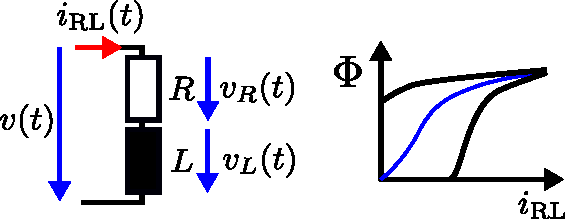
\includegraphics[width=0.5\linewidth]{Abbildungen/Modellbildung/PDF/RLglied.pdf}
	\caption{Reihenschaltung aus Induktivität und Widerstand}
	\label{fig:rlglied}
\end{figure}
%  
Unter Berücksichtigung der Eisensättigung der realen Induktivität würde sich für den magnetischen Fluss eine exemplarische nichtlineare Kurve, wie in Abbildung~\ref{fig:rlglied} ergeben.
Im ersten Schritt werden nun die mathematischen Gleichungen des Systems beginnend mit dem Maschensatz aufgestellt \eqref{eq:diffglrl}.
%
\begin{equation}
\begin{aligned}
	&v(t)=v_{\text{R}}(t)+v_{\text{L}}(t).\\
\end{aligned}
\end{equation}
%
Danach können die Gleichungen für die einzelnen Elemente aufgestellt werden
%
\begin{equation}
\begin{aligned}	
	&v_{\text{R}}(t) = R\cdot i_{\text{RL}}(t)\\
	&v_{\text{L}}(t) = \frac{\text{d}\Phi(t)}{\text{d}t}\\
	&i_{\text{RL}}(t) = f\left(\Phi(t)\right) &&\text{Nichtlinear Zusammenhang}\label{eq:diffglrl}
\end{aligned}
\end{equation}
%
Im zweiten Schritt können die aufgestellten Systemgleichungen in einzelnen Blöcken grafisch dargestellt und zusammengeführt werden. Dies erleichtert die spätere Darstellung im sogenannten Blockschaltbild. Zunächst muss jedoch noch definiert werden welche Größe den Eingang und welche den Ausgang des Systems beschreiben soll. In diesem Beispiel nutzen wir $v(t)$ als Eingang, das dieser direkt im System beeinflussbar ist und $i_{\text{RL}}(t)$ als Ausgang. Alle Gleichungen aus \eqref{eq:diffglrl} werden einem Block zugeordnet und ergeben folgende Schaltbilder:
%
%\begin{figure}[h]
%	\begin{minipage}{0.5\textwidth}
%	\begin{itemize}
%		\item Kennlinienglied $i_{\text{RL}}=f(\Phi(t))$
%	\end{itemize}
%	Kennlinienglieder beschreiben einen statischen funktionalen Zusammenhang zwischen Eingang und Ausgang (in der Regel nichtlinear).
%	\end{minipage}\hfill
%	\begin{minipage}{0.5\textwidth}
%		\centering
%		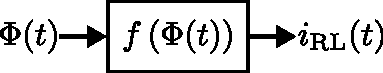
\includegraphics[width=0.7\textwidth]{Abbildungen/Modellbildung/PDF/Kennlinienglied.pdf}
%	\end{minipage}
%\end{figure}
%%
%  \begin{figure}[h]
%	\begin{minipage}{0.5\textwidth}
%		\begin{itemize}
%			\item Proportionalglied $v_{\text{R}}=R\cdot i_{\text{RL}}$
%		\end{itemize}
%		Proportionalglieder beschreiben einen statischen funktionalen Zusammenhang zwischen Eingang und Ausgang (linearer Fall).
%	\end{minipage}
%	\begin{minipage}{0.5\textwidth}
%		\centering
%		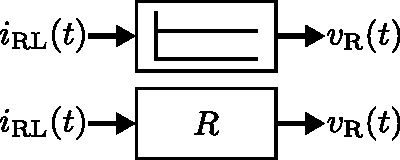
\includegraphics[width=0.7\textwidth]{Abbildungen/Modellbildung/PDF/Proportionalglied.pdf}
%	\end{minipage}
%\end{figure} 
%%
%  \begin{figure}[h]
%	\begin{minipage}{0.5\textwidth}
%		\begin{itemize}
%			\item Differentationsglied $v_{\text{L}}=\frac{\text{d}\Phi(t)}{\text{d}t}$
%		\end{itemize}
%		Berechnet die Ableitung des Eingangsignals und stellt es am Ausgang bereit.
%	\end{minipage}\hfill
%	\begin{minipage}{0.5\textwidth}
%		\centering
%		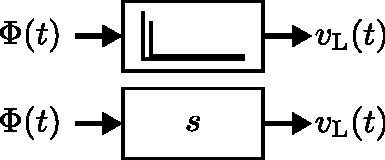
\includegraphics[width=0.7\textwidth]{Abbildungen/Modellbildung/PDF/Differnzierglied.pdf}
%	\end{minipage}
%\end{figure} 
%%
%  \begin{figure}[h]
%	\begin{minipage}{0.5\textwidth}
%		\begin{itemize}
%			\item Integrationsglied $\Phi =\frac{1}{T}\int v_{\text{L}}(t)\text{d}t$
%		\end{itemize}
%	Integrationsglieder integrieren den Systemeingang auf und bilden daraus den Systemausgang. Die Variable $T$ gibt die Integrationszeitkonstante an.
%	\end{minipage}\hfill
%	\begin{minipage}{0.5\textwidth}
%		\centering
%		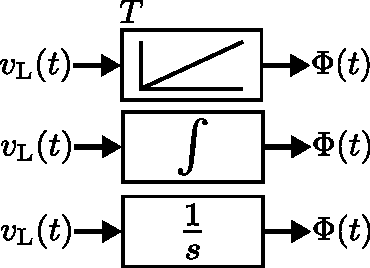
\includegraphics[width=0.7\textwidth]{Abbildungen/Modellbildung/PDF/Integratorglied.pdf}
%	\end{minipage}
%\end{figure} 
%%
%  \begin{figure}[h]
%	\begin{minipage}{0.5\textwidth}
%		\begin{itemize}
%			\item Summationsglied $v_{\text{L}}=v-v_{\text{R}}$
%		\end{itemize}
%		Durch ein Summationsglied kann die Addition oder Subtraktion zweier Größen dargestellt werden.
%	\end{minipage}\hfill
%	\begin{minipage}{0.5\textwidth}
%		\centering
%		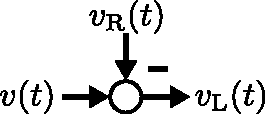
\includegraphics[width=0.5\textwidth]{Abbildungen/Modellbildung/PDF/Summationsglied.pdf}
%	\end{minipage}
%\end{figure}
%

\begin{figure}[h]
  \begin{subfigure}[c]{\textwidth}
	\begin{minipage}{0.5\textwidth}
	\begin{itemize}
		\item Kennlinienglied $i_{\text{RL}}=f(\Phi(t))$
	\end{itemize}
	Kennlinienglieder beschreiben einen statischen funktionalen Zusammenhang zwischen Eingang und Ausgang (in der Regel nichtlinear).
	\end{minipage}\hfill
	\begin{minipage}{0.5\textwidth}
		\centering
		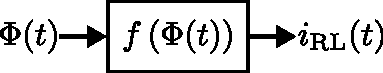
\includegraphics[width=0.7\textwidth]{Abbildungen/Modellbildung/PDF/Kennlinienglied.pdf}
	\end{minipage}
\end{subfigure}
%
%\vspace{1cm}
%
  \begin{subfigure}[c]{\textwidth}
	\begin{minipage}{0.5\textwidth}
		\begin{itemize}
			\item Proportionalglied $v_{\text{R}}=R\cdot i_{\text{RL}}$
		\end{itemize}
		Proportionalglieder beschreiben einen statischen funktionalen Zusammenhang zwischen Eingang und Ausgang (linearer Fall).
	\end{minipage}
	\begin{minipage}{0.5\textwidth}
		\centering
		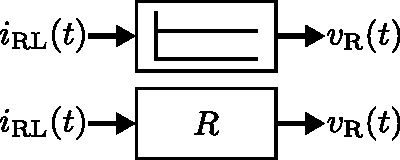
\includegraphics[width=0.7\textwidth]{Abbildungen/Modellbildung/PDF/Proportionalglied.pdf}
	\end{minipage}
\end{subfigure} 
%
%\vspace{0.5cm}
%
  \begin{subfigure}[c]{\textwidth}
	\begin{minipage}{0.5\textwidth}
		\begin{itemize}
			\item Differentationsglied $v_{\text{L}}=\frac{\text{d}\Phi(t)}{\text{d}t}$
		\end{itemize}
		Berechnet die Ableitung des Eingangsignals und stellt es am Ausgang bereit.
	\end{minipage}\hfill
	\begin{minipage}{0.5\textwidth}
		\centering
		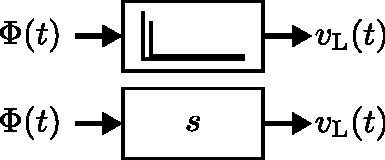
\includegraphics[width=0.7\textwidth]{Abbildungen/Modellbildung/PDF/Differnzierglied.pdf}
	\end{minipage}
\end{subfigure} 
%
%\vspace{1cm}
%
  \begin{subfigure}[c]{\textwidth}
	\begin{minipage}{0.5\textwidth}
		\begin{itemize}
			\item Integrationsglied $\Phi =\frac{1}{T}\int v_{\text{L}}(t)\text{d}t$
		\end{itemize}
	Integrationsglieder integrieren den Systemeingang auf und bilden daraus den Systemausgang. Die Variable $T$ gibt die Integrationszeitkonstante an.
	\end{minipage}\hfill
	\begin{minipage}{0.5\textwidth}
		\centering
		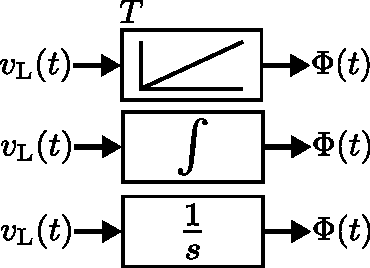
\includegraphics[width=0.7\textwidth]{Abbildungen/Modellbildung/PDF/Integratorglied.pdf}
	\end{minipage}
\end{subfigure} 
%
%\vspace{1cm}
%
  \begin{subfigure}[c]{\textwidth}
	\begin{minipage}{0.5\textwidth}
		\begin{itemize}
			\item Summationsglied $v_{\text{L}}=v-v_{\text{R}}$
		\end{itemize}
		Durch ein Summationsglied kann die Addition oder Subtraktion zweier Größen dargestellt werden.
	\end{minipage}\hfill
	\begin{minipage}{0.5\textwidth}
		\centering
		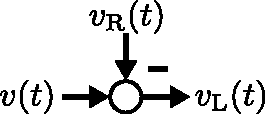
\includegraphics[width=0.5\textwidth]{Abbildungen/Modellbildung/PDF/Summationsglied.pdf}
	\end{minipage}
\end{subfigure}
\end{figure}
%
%\newpage
%
Durch Kombination der einzelnen Blöcke können nun die Gleichungen aus \eqref{eq:diffglrl} als Blockschaltbild dargestellt werden (Abbildung~\ref{fig:blockschaltbild}).
%
\begin{figure}[h]
	\centering
	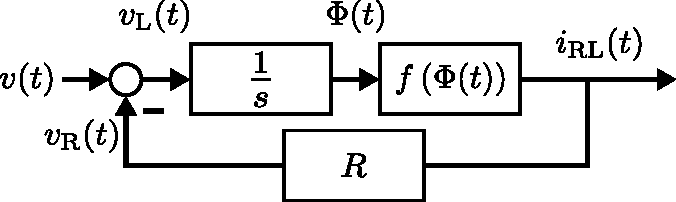
\includegraphics[width=0.65\linewidth]{Abbildungen/Modellbildung/PDF/Wirkschaltplan.pdf}
	\caption{Wirkschaltplan des dynamischen Verhaltens des RL-Glieds (vgl. \cite{Foellinger94})}
	\label{fig:blockschaltbild}
\end{figure}
%
Dieses erste anschauliche Beispiel hat nun vier Übertragungsglieder eingeführt, welche in der Darstellung von technischen Systemen genutzt werden können. Die Kennlinien in den Blöcken stellen die Antwort des Block Ausgangs auf einen Sprung am Eingang dar. Es stellt sich jedoch die Frage, wie Übertragungsglieder etwas allgemeiner klassifiziert werden können. Hierzu sollen die wichtigsten Merkmale im nächsten Kapitel dargestellt werden.
%
%##############################################################################
\section{Klassifikation von Übertragungsgliedern}
%##############################################################################
%
Ein Übertragungsglied beschreibt eine mathematische Abbildung zwischen Eingangsgröße $u(t)$ und Ausgangsgröße $y(t)$. Die Abbildung kann eine allgemeine Funktion sein z.B. $y(t)=u^{3}(t)$ aber eben auch eine Differentialgleichung. Letzteres bezieht sich auf den Fall, dass ein dynamisches System durch ein Übertragungsglied dargestellt werden soll. Übertragungsglieder können durch eindeutige Eigenschaften klassifiziert werden \cite{Foellinger94, Unbehauen08, Lunze10, Zacher17}, welche im Folgenden näher erläutert werden.
%
%##############################################################################
\subsection{Dynamik}
%##############################################################################
%
Wie schon im einführenden Beispiel (Abbildung~\ref{fig:rlglied}) dargestellt gibt es dynamische und statische Anteile in einem technischen System. Statische Anteile sind z.B.
%
\begin{itemize}
	\item Kennlinien für Magnetisierung, Materialfestigkeit, Federsteifigkeit, Reibkonstante (Reifen Bodenkontakt) etc.
	\item Falls die Dynamik eines Teilsystems wesentlich kleinere Zeitkonstanten aufweist, wie die anderen betrachteten Elemente und deren Einfluss auf das Gesamtverhalten vernachlässigbar ist. In diesem Fall wird meist nur die statische Verstärkung ($h(t)$ für $t\rightarrow \infty$) des vormals dynamischen Teilsystems betrachtet.
\end{itemize}
%
Im Falle eines statischen Anteils ist die Abbildung zwischen Ein- und Ausgang konstant und nicht von weiteren Einflussgrößen Abhängig. Dies ist beispielsweise ein Ansatz, wenn Dynamiken des betrachteten technischen Systems so schnell ablaufen, dass sie für deren Modellierung keine Rolle spielen. Bei einem dynamischen Übertragungsglied kann sich die Übertragungseigenschaft zwischen Ein- und Ausgang ändern. Grund für eine Systemdynamik sind die Energiespeicher in einem technischen System. Energiespeicher bewirken das einzelne Systemgrößen wie Spannung $v(t)$ oder Strom $i(t)$ sich nicht schlagartig ändern können. So ist beispielsweise in einer realen Induktivität Energie im magnetischen Feld gespeichert. Bei einer konstanten Eingangspannung würde nach \eqref{eq:diffglrl} der magnetische Fluß $\Phi$ linear, jedoch niemals sprungförmig ansteigen.
%
%############################################################################
\subsection{Linearität}
%############################################################################
%
Die Linearität ist die wichtigste Eigenschaft der in dieser Vorlesung untersuchten Klasse von Systemen. 
%
\subsubsection{Lineare Übertragungsglieder}
%
Grundsätzlich gehorchen lineare Systeme zwei wesentlichen Eigenschaften. Zum einen gilt das Superpositions- oder Überlagerungsprinzip \eqref{eq:superpos}.
%
\begin{equation}
y(t) = f((u_{1}(t)+u_{2}(t))=f(u_{1}(t))+f(u_{2}(t))\label{eq:superpos}
\end{equation}
%
In Form eines Blockschaltbildes bedeutet dies, dass die Summationsstelle der Eingangsgrößen verschoben werden kann, jedoch die selbe Ausgangsgröße entsteht (Abbildung~\ref{fig:blockschaltbildsumme}). Diese Eigenschaft wird auch \textbf{Additivität} genannt. 
%
\begin{figure}[h]
	\centering
	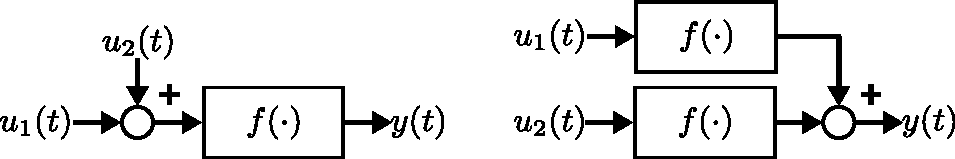
\includegraphics[width=0.8\linewidth]{Abbildungen/Modellbildung/PDF/Summation_Linearitaet.pdf}
	\caption{Vertauschung der Summationstelle bei linearen Übertragungsliedern}
	\label{fig:blockschaltbildsumme}
\end{figure}
%
Die zweite wesentliche Eigenschaft von linearen Systemen ist die \textbf{Homogenität}. Diese beschreibt, dass sich konstante Verstärkungsfaktoren aus einer Funktion ausklammern lassen, ohne, dass sich hierdurch deren Wirkung auf den Systemausgang verändern \eqref{eq:homogen}. 
%
\begin{equation}
y(t) = f\left(ku_{1}(t)\right)=kf\left(u_{1}(t)\right)\label{eq:homogen}
\end{equation}
%
Es ist möglich diesen Zusammenhang wieder in einem Blockschaltbid darzustellen (Abbildung~\ref{fig:blockschaltbildhomogen}). 
%
\begin{figure}[h]
	\centering
	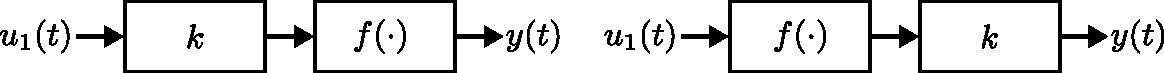
\includegraphics[width=0.9\linewidth]{Abbildungen/Modellbildung/PDF/Homogenitaet.pdf}
	\caption{Vertauschung der konstanten Verstärkungsfaktoren bei linearen Übertragungsliedern}
	\label{fig:blockschaltbildhomogen}
\end{figure}
%
Es lässt sich als Merkregel festhalten: Ist eine Funktion aus einer Summe lineare Übertragungsglieder entstanden, so ist die Funktion selbst wieder linear. 
%
\begin{Aufgaben}{}{}
	\begin{itemize}
		\item \textit{Linearitätsnachweis bei Integratorketten}
		\item \textit{Linearitätsnachweis von MIMO Summationsgliedern}
	\end{itemize}
\end{Aufgaben}
%
\subsubsection{Nichtlineare Übertragunsglieder}
%
Untersucht man nichtlineare Übertragungsglieder so sind die Beiden vorgenannten Eigenschaften nicht vorzufinden. Als einfaches Beispiel lässt sich hier die Multiplikation von zwei Größen darstellen \eqref{eq:multiplikation}
%
\begin{equation}
y(t) = f\left(u_{1}(t),u_{2}(t)\right)=u_{1}(t)\cdot u_{2}(t) \label{eq:multiplikation}
\end{equation}
%
Nehmen wir nun Verstärkungsfaktoren hinzu
%
%
\begin{equation*}
\begin{aligned}
u_{1}(t)&=\hat{k}\hat{u}_{1}(t)+\tilde{k}\tilde{u}_{1}(t)\\
u_{2}(t)&=\hat{k}\hat{u}_{2}(t)+\tilde{k}\tilde{u}_{2}(t)\\
y(t)&=f\left(\hat{k}\,\hat{u}_{1}(t)+\tilde{k}\tilde{u}_{1}(t),\hat{k}\,\hat{u}_{2}(t)+\tilde{k}\tilde{u}_{2}(t)\right)=\left(\hat{k}\,\hat{u}_{1}(t)(t)+\tilde{k}\tilde{u}_{1}(t)\right)\left(\hat{k}\,\hat{u}_{2}(t)+\tilde{k}\tilde{u}_{2}(t)\right)\\
	&= k^{2}\,\hat{u}_{1}(t)\hat{u}_{2}(t)+\tilde{k}^{2}\tilde{u}_{1}(t)\tilde{u}_{2}(t)+\hat{k}\tilde{k}\hat{u}_{1}(t)\tilde{u}_{2}(t)+\hat{k}\tilde{k}\tilde{u}_{1}(t)\hat{u}_{2}(t)\\
\end{aligned}
\end{equation*}
%
wird die Homogenitätsbedingung in diesem Fall nicht erfüllt. Es kann kein konstanter Verstärkungsfaktor $k$ oder $\tilde{k}$ ausgeklammert werden. Ein weiteres Beispiel stellt eine Kennlinie dar. 
%
\begin{figure}[h]
	\centering
	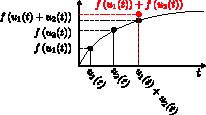
\includegraphics[width=0.6\linewidth]{Abbildungen/Modellbildung/PDF/NichtlinKurve.pdf}
	\caption{Nichtlineare Kennlinie zur Darstellung der Nichtlinearität}
	\label{fig:nichtlinkurve}
\end{figure}
%
Trägt man Werte auf der horizontalen Achse mit gleichem Abstand auf, so ist addiert sich nicht zwingend auch der Funktionswert, wie in Abbildung~\ref{fig:nichtlinkurve} dargestellt. Es ist zu erkennen das die Eigenschaft der Additivität nicht erfüllt ist denn
%
\begin{equation*}
\begin{aligned}
f\left(u_{1}(t)+u_{2}(t)\right)\neq f\left(u_{1}(t)\right)+f\left(u_{2}(t)\right).\\
\end{aligned}
\end{equation*}
%
Grundsätzlich existiert für nichtlineare Systeme in der Regelungstechnik immer noch keine vollständig zusammenhängende Theorie \cite{Adamy09}. Es existieren zudem nicht so zusammenhängende und gut strukturierte Entwurfsverfahren für Regler (mit einigen Ausnahmen).
Die Untersuchung der Stabilität ist ein weiteres Themenfeld, welches in der nichtlinearen Regelungstechnik schwierig zu behandeln ist.
Nichtlineare System werden deshalb in den meisten praktischen Anwendungsfällen durch eine Linearisierung im Arbeitspunkt 'umgewandelt'. Ihr Verhalten kann dann nahe dieses Arbeitspunktes ausreichen gut druch das Ersatzmodell nachgebildet werden und Entwurfsmethoden für lineare Systeme kommen zum Einsatz.
%
\subsection{Zeitinvarianz}
%
Formal lässt sich die Zeitinvarianz eines Systems durch eine Unabhängigkeit der zeitlichen Verschiebung klassifizieren \cite{Foellinger94,Lunze10} \eqref{eq:verschiebungssatz}.
%
\begin{equation}
\begin{aligned}
y(t)&=f\left(u(t)\right)\\
y(t-T)&=f\left(u(t-T)\right)\label{eq:verschiebungssatz}
\end{aligned}
\end{equation}
%
Dies bedeutet, dass sich die Systemantwort eines zeitinvarianten Systems auf einen identischen Eingang (bei gleichem Anfangswert!) immer gleich Verhalten wird, unabhängig davon wann die Anregung durch den Eingang erfolgt.
%
\begin{figure}[h]
	\centering
	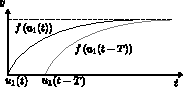
\includegraphics[width=0.55\linewidth]{Abbildungen/Modellbildung/PDF/Zeitinvariant.pdf}
	\caption{Beispielhafte Darstellung des Verschiebungssatzes}
	\label{fig:zeitinvariant}
\end{figure}
%
In Abbildung~\ref{fig:zeitinvariant} ist die Sprungantwort eines zeitinvarianten System dargestellt. Es ist deutlich erkennbar, das sowohl die Kurvenform als auch der Endwert sich nicht unterscheiden. Wenn ein System sowohl linear als  auch zeitinvariant ist, dann spricht man oft von sogenannten 'LZI-System' (lineare und zeitinvariante Systeme) oder Englisch 'LTI-systems' (linear and time-invariant systems). In dieser Vorlesung wird dies die Systemklasse sein, mit der wir uns hauptsächlich beschäftigen.
%
\subsubsection{Beispiele für zeitvariante Systeme}
%
Zeitvariante Systeme sind in der Praxis oft vorzufinden. Ein Beispiel sind zeitlich veränderliche Parameter \cite{Unbehauen08}
\begin{itemize}
	\item Rakete (Massenänderungen des Treibstoffs während des Flugs)
	\item Gleichstrommaschine (temperaturabhängiger Widerstand der Ankerwicklung, welcher sich durch Belastung erwärmt)
\end{itemize}
%
Ein weiteres Beispiel ist das Abtast-Halte-Glied, welches in der zeit-diskreten Regelung zur Wandlug von analogen Signalen genutzt wird. Dieses misst die Regelgröße $y(t)$ in äquidistanten (konstanter Abstand) Zeitpunkten \cite{Foellinger94} und hält den gemessenen Wert als $\overline{y}(\tau)$ für einen konstanten Zeitraum $t_{i}$ fest, wie in Abbildung~\ref{fig:abtastglied} in schwarz dargestellt.
%
\begin{figure}[h]
	\centering
	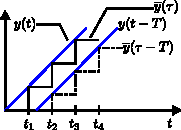
\includegraphics[width=0.4\linewidth]{Abbildungen/Modellbildung/PDF/Abtastglied.pdf}
	\caption{Untersuchung zum Verschiebungssatz bei einem Abtastglied}
	\label{fig:abtastglied}
\end{figure}
%
Dieses Halteglied bereitet somit ein physisches Signal z.B. für einen Microcontroller auf, in dem die Verarbeitung nicht kontinuierlich stattfindet, sondern in diskreten Zeitabständen. \underline{Hinweis:} Das Abtast-Halteglied misst und speichert den kontinuierlichen Wert (Abbildung~\ref{fig:abtastglied} in blau) bis zum nächsten Abtastzeitpunkt $t$ und übernimmt dann den Neuen gemessenen. Diese Glied ist somit zwar linear aber nicht zeitinvariant.
%
%
\begin{Aufgaben}{}{}
	\begin{itemize}
		\item \textit{PWM Stromregelung Gleichstromsteller}
	\end{itemize}
\end{Aufgaben}
%
\subsection{Kausalität}
%
Die Kausalität eines Systems beschreibt, das Eingangsgrößen zum aktuellen Zeitpunkt bspw. $t=0$ den Ausgang nur für zukünftige Zeitpunkte beeinflussen können \cite{Lunze10}. Praktische Systeme sind immer kausal, weshalb diese Eigenschaft in der Vorlesung nicht weiter behandelt werden soll. 
%
%############################################################################
\section{Beschreibung lineare Systeme im Zeitbereich}
%############################################################################
%
%############################################################################
\subsection{Beschreibung lineare Systeme durch Differenzialgleichungen}
%############################################################################
%
Ob ein System durch ein Blockschaltbild oder eine Differentialgleichung dargestellt wird ist grundsätzlich gleichwertig \cite{Ament17}. In der Regel macht sich die Modellbildung die physikalischen Gesetzmäßigkeiten zu nutze und leitet aus ihnen die mathematischen Differenzialgleichungen ab, welche das untersuchte technische System beschreiben. Im folgenden sind die physikalischen Prinzipien, welche für die meisten Systeme ausreichend sind, genannt \cite{Ament17}
\begin{itemize}
	\item Mechanik: also Newtonsche Bewegungseichungen.
	\item Elektrische Systeme: Sätze von Kirchhoff, Strom-Spannungsbeziehung elektrischer Bauteile.
	\item Chemie und Biologie: Bilanzgleichungen für Volumen, Stoff, Massen.
	\item Thermodynamik: Temperatur, Innere Energie, Kreisprozesse
\end{itemize}
%
Formuliert man diese nun zusammen mit deren zeitlichen oder räumlichen Beziehungen zueinander, erhält man die beschreibenden Differenzialgleichungen des Systems.
%
%############################################################################
\subsubsection{Aufstellen und lösen der linearen Differenzialgleichung}
%############################################################################
%
Das Aufstellen und Lösen von Differenzialgleichungen wurde in anderen Grundlagenvorlesungen bereits behandelt, soll hier aber der Vollständigkeit halber nochmals in kurzer Form aufgezeigt werden. Zunächst gehen wir von einer allgemeinen linearen Differenzialgleichung (LDGL) mit konstanten Koeffizienten aus. Diese stellen sich in dieser Vorlesung in folgender Form dar (vgl. Gleichung~\ref{eq:lindgl})
%
\begin{equation}
\begin{aligned}
a_{n}\frac{\text{d}^{n}y}{\text{d}t^{n}}+&a_{n-1}\frac{\text{d}^{n-1}y}{\text{d}t^{n-1}}+\cdots+a_{1}\frac{\text{d}y}{\text{d}t}+a_{0}y=\\
&b_{q}\frac{\text{d}^{q}u}{\text{d}t^{q}}+b_{q-1}\frac{\text{d}^{q-1}u}{\text{d}t^{q-1}}+\cdots+b_{1}\frac{\text{d}u}{\text{d}t}+b_{0}u\label{eq:lindgl}
\end{aligned}
\end{equation}
%
Mit ${a_{0},\dots,a_{n}}$ die konstanten Koeffizienten der linken Seite (Ausgang) und ${b_{0},\dots,b_{n}}$ die konstanten Koeffizienten der rechten Seite (Eingang). Die Variablen $q$ und $n$ stellen jeweils die Höhe der Ableitungen dar. Für diese (LDGL) müssen wir nun, um die homogene Lösung (Eigendynamik oder Eigenbewegung) zu finden, die rechte Seite zu null setzten. Die rechte Seite beschreibt den Eingang auf das System bzw. die Anregung von Außen. 
%
\begin{equation}
\begin{aligned}
&a_{n}\frac{\text{d}^{n}y}{\text{d}t^{n}}+a_{n-1}\frac{\text{d}^{n-1}y}{\text{d}t^{n-1}}+\cdots+a_{1}\frac{\text{d}y}{\text{d}t}+a_{0}y=0 \label{eq:homdgl}
\end{aligned}
\end{equation}
%
Um die LDGL zu lösen wird die charakteristische Gleichung aufgestellt und deren Wurzeln bestimmt. Dabei gilt die Regel: $\frac{\text{d}^{n}y}{\text{d}t^{n}}=\lambda^{n}$. Beim letzten Element setzt man folglich $\frac{\text{d}^{0}y}{\text{d}t^{0}}=1$ (wenn auch mathematisch nicht vollständig korrekt, ist es so leicht zu merken).
%
\begin{equation}
\begin{aligned}
&a_{n}\lambda^{n}+a_{n-1}\lambda^{n-1}+\cdots+a_{1}\lambda+a_{0}=0 \label{eq:characterrischegl}
\end{aligned}
\end{equation}
%
Anschließend wird die Lösung des Polynoms \eqref{eq:characterrischegl} ermittelt. Diese Lösung kann man bei Polynomen mit $n=3$ oder $n<3$ per Hand bestimmen, jedoch werden in der Praxis auch hier meist numerische Verfahren genutzt \cite{Lunze10} \cite{Bruen21}, um die Wurzeln zu bestimmen. Wenn die Wurzeln bestimmt wurden, werden Ansatzfunktionen genutzt, um eine Zeitfunktion für die homogene Lösung zu ermitteln. Falls alle Lösungen $\lambda_{k}=\delta_{k}$ reellwertig sind und nicht doppelt $\delta_{k}\neq\delta_{k+1}$ vorkommen, wird eine Summe aus Exponentialfunktionen genutzt.
%
\begin{equation}
\begin{aligned}
&y_{\text{hom}}(t)=\sum_{k=1}^{N}c_{k}e^{\delta_{k}t}\label{eq:dglloesungreel}
\end{aligned}
\end{equation}
%
Falls es sich um ein schwingungsfähiges System handelt, d.h. es existieren Lösungen für die Wurzeln in Form von $\lambda_{k}=\delta_{k}\pm j\omega_{k}$, wobei $j$ die imaginäre Einheit ist, muss dieser schwingungsfähige Anteil in der Lösung berücksichtigt werden.
%
\begin{equation}
\begin{aligned}
&y_{\text{hom}}(t)=\sum_{k=1}^{N}c_{k}e^{\delta_{k}t}+\sum_{l=1}^{L}e^{\delta_{l}t}\left[c_{1,l}\cos(\omega_{l}t)+c_{2,l}\sin(\omega_{l}t)\right]\label{eq:dglloesungkomplex}
\end{aligned}
\end{equation}
%
%Durch einsetzten der Lösung in Gleichung~\ref{eq:characterrischegl} lassen sich über Koeffizientenvergleich, die Vorfaktoren $c_{k}, c_{l} \forall k,l \in N,L$ in Gleichung~\ref{eq:dglloesungreel} und \ref{eq:dglloesungkomplex} bestimmen.\\

Der zweite Schritt beinhaltet das Auffinden der partikulären Lösung, welche je nach Eingangssignal einen anderen Ansatz besitzt. Eine gute Zusammenfassung verschiedener Ansätze ist in \cite{Furlan08,Gangster03} zu finden. Die wichtigsten Ansätze für die Regelungstechnik sind:
%
\begin{equation}
\begin{aligned}
&u(t) = A, &&\text{Ansatz} \rightarrow y_{\text{part}}(t) = B\\
&u(t) = t^{m}, &&\text{Ansatz} \rightarrow y_{\text{part}}(t) = A_{0}+A_{1}t+\ldots+A_{m}t^{m}\\
&u(t) = A\sin(\omega t), &&\text{Ansatz} \rightarrow y_{\text{part}}(t) = C\sin(\omega t)+D\cos(\omega t)
\end{aligned}
\end{equation}
%
Nachdem der partikuläre Lösungsansatz auswählt wurde, wird dieser in Gleichung~\ref{eq:lindgl} eingesetzt (Ableitungen beachten!) und durch Koeffizientenvergleich die Vorfaktoren ermittelt. Die allgemeine Lösung der Differenzialgleichung ergibt sich aus der Summe von homogener und partikulärer Lösung.
%
\begin{equation}
\begin{aligned}
&y(t)=y_{\text{hom}}(t)+y_{\text{part}}(t)
\end{aligned}
\end{equation}
%
Um die allgemeine Lösung der DGL nun zu bestimmen, müssen Anfangswerte oder allgemein Randwerte der DGL bekannt sein. Dies könnte z.B. die Anfangsauslegung eines Systems sein. Anfangswerte werden benötigt, um die konstanten Koeffizienten der allgemeinen Lösung des homogenen Anteils zu errechnen. Durch Einsetzten der Anfangswerte lassen sich diese wieder durch einen Koeffizientenvergleich bestimmen.
%
Zusammengefasst ergeben sich für die Vorgehensweise beim lösen der DGL:
\begin{itemize}
	\item Auffinden der freien Bewegung (homogene Lösung)
	\item Bestimmung der erzwungenen Bewegung (partikuläre Lösung)
	\item Aufstellen der allgemeinen Lösung
	\item Lösungen des Anfangswertproblems 
\end{itemize}
%
\begin{Aufgaben}{}{}
	\begin{itemize}
		\item \textit{Beispielhafte Lösung der DGL eines mechanischen Systems 2ter-Ordnung}
	\end{itemize}
\end{Aufgaben}
%
%%############################################################################
%\subsubsection{Beispielhafte Lösung eines mechanischen Systems}
%%############################################################################
%%
%Beispielhaft soll hier ein mechanisches System bestehend aus Masse, Dämpfer und einer Feder beschrieben werden, wie in Abbildung~\ref{fig:federmassedaempfer} dargestellt. Dieses System lässt sich als lineare Differentialgleichung zweiter Ordnung beschreiben und für den homogenen Fall folgendermaßen aufstellen \eqref{eq:massedgl}:
%%
%\begin{equation*}
%\begin{aligned}
%m\cdot \frac{\text{d}^{2}x(t)}{\text{d}t^{2}} + d\cdot \frac{\text{d}x(t)}{\text{d}t} + c x(t)=F_{g}\cdot\sin(t)\label{eq:massedgl}
%\end{aligned}
%\end{equation*}
%%
%Um diese LDGL zu lösen nehmen wir zunächst an, dass es sich um ein schwingungsfähiges System handelt, d.h. wir haben eine Lösung der charakteristischen Gleichung der Form $s_{k}=\delta_{k}\pm j\omega_{k}$. Diese setzten wir ein und bekommen
%%
%\begin{equation*}
%\begin{aligned}
%&x_{\text{hom}}(t)=e^{\delta_{l}t}\left[c_{1,l}\cos(\omega_{e}t)+c_{2,l}\sin(\omega_{e}t)\right]
%\end{aligned}
%\end{equation*}
%%
%Die beiden Faktoren $\delta$ und $\omega_{\text{e}}$ erhalten wir aus der Lösung der charakteristischen Gleichung:
%%
%\begin{equation*}
%\begin{aligned}
%&\lambda^{2}+\frac{d}{m}\lambda+\frac{c}{m}=0\\
%&\lambda_{1,2} = \underbrace{-\frac{d}{2m}}_{\delta}\pm \underbrace{\sqrt{\left(\frac{d}{2m}\right)^{2}-\frac{c}{m}}}_{\omega_{\text{e}}}
%\end{aligned}
%\end{equation*}
%%
%Die partikuläre Lösung ergibt sich unter Annahme eines Einheitssprung als Eingang allgemein zu 
%%
%\begin{equation*}
%\begin{aligned}
%%x_{\text{part}}(t)&=\sum_{k=1}^{N}c_{k}(t)x_{k}(t)\\
%x_{\text{part}}(t)&=1
%\end{aligned}
%\end{equation*}
%%
%\eqref{eq:dglloesung} zu
%%
%\begin{equation*}
%\begin{aligned}
%x(t)&=K\left[1 -\frac{1}{\sqrt{1-D^{2}}}\cdot e^{-D\omega_{0}t}\cdot\sin\left(\omega_{e}t+\text{arcos}(D)\right)\right]\\
%&\omega_{e} = \omega_{0}\sqrt{1-D^{2}}
%\end{aligned}
%\end{equation*}
%%
%Das durch diese Differenzialgleichung beschriebene Verhalten wird in Abbildung~\ref{fig:federmassedaempfer} für die Auslenkung um eine Gleichgewichtslage dargestellt. 
%%
%\begin{figure}[h]
%	\centering
%	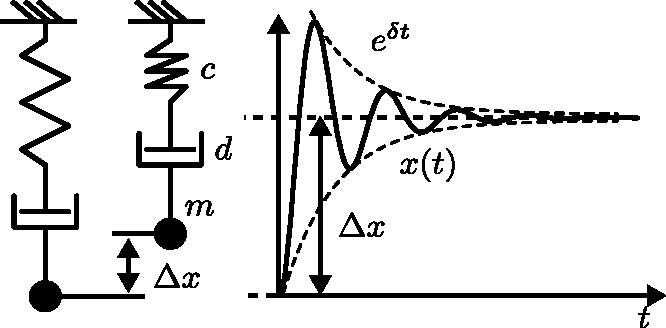
\includegraphics[width=0.65\linewidth]{Abbildungen/Modellbildung/PDF/MasseFederDaempfer.pdf}
%	\caption{Feder, Masse, Dämpfer System und dessen Verhalten bei Auslenkung um eine Gleichgewichtslage}
%	\label{fig:federmassedaempfer}
%\end{figure}  
%%
%############################################################################
\subsubsection{Gewichtsfunktion und Faltung}
%############################################################################
%
Im vorherigen Beispiel haben wir die Auffindung der allgemeinen Lösung einer linearen Differenzialgleichung für ein mechanisches Teilsystem aufgezeigt. Es existiert im Grunde hierfür auch eine kompaktere Schreibweise, denn ein System kann durch eine Lösung der allgemeinen DGL dargestellt werden, welche sich für verschwindende Anfangswerte $y(0)=0$ ergibt. Durch den Anfangswert 0 ist das System in Ruhe und wird nur durch die Anregung eines Eingangssignals aus der Ruhelage ausgelenkt. Das sogenannte Übertragungsverhalten klassifiziert ein dynamisches Systems. Dies bedeutet, dass das System bei verschwindenden Anfangsbedingungen durch sein Ein- Ausgangsverhalten eindeutig beschrieben wird. Die sich ergebende Zeitfunktion wird dann als Gewichtsfunktion $g(t)$ eines dynamischen Systems bezeichnet. Das Systemverhalten auf ein Eingangssignal ergibt sich durch die Berechnung des folgenden Integrals. 
%
\begin{equation}
\begin{aligned}
&y(t)=\int_{0}^{t_{0}}g(t)u(t_{0}-t)\text{d}t\label{eq:faltung}
\end{aligned}
\end{equation}
%
Das Integral \eqref{eq:faltung} wird auch als Faltungsintegral bezeichnet. Die Gewichtsfunktion gibt an, wie stark ein vergangener Wert des Eingangs $u(t_{0}-t)$ durch das Systemverhalten (beschrieben durch $g(t)$) gewichtet wird und somit auf den Ausgang $y(t)$ wirkt. Diese Beschreibung wird in der Literatur auch in folgender Weise dargestellt:
%
\begin{equation}
\begin{aligned}
&y(t)=g(t)*u(t)
\end{aligned}
\end{equation}
%
Grundsätzlich kann man mit dieser Formulierung die Systemantwort eines dynamischen Systems für beliebige Eingangssignale berechnen. Jedoch ist diese Schreibweise trotz allem sehr abstrakt und soll nachfolgend konkretisiert werden. 
%
%############################################################################
\subsubsection{Einheitssprung und Sprungantwort}
%############################################################################
%
In der Regelungstechnik wird zur Anregung des Eingangs eines Systems meist der Einheitssprung (auch Heaviside-Funktion genannt) heran gezogen, welcher durch folgende Beziehung beschrieben wird:
%
\begin{equation}
\begin{aligned}
u(t)=\sigma(t)=\begin{cases}
0  & \text{ falls } t < 0 \\
1  & \text{ falls } t \ge 0 \\
\end{cases}& \label{eq:einheitssprung}
\end{aligned}
\end{equation}
%
Die Sprungantwort $h(t)$ eines Systems beschreibt die Antwort des jeweiligen Systems auf einen Einheitssprung
%
\begin{equation}
\begin{aligned}
&h(t)=\int_{0}^{t_{0}}g(t)\underbrace{\sigma(t_{0}-t)}_{=1}\text{d}t\\
&h(t)=\int_{0}^{t_{0}}g(t)\text{d}t \label{eq:sprungantwort}
\end{aligned}
\end{equation}
%
Somit ist die Sprungantwort $h(t)$ das Integral der Gewichtsfunktion $g(t)$. Dies stellt zusammen mit der Impulsantwort einen wichtigen Zusammenhang in der Regelungstechnik dar. Die Impulsantwort ist definiert als die Antwort des Systems auf einen Einheitsimpuls und wird direkt durch die Gewichtsfunktion $g(t)$ beschrieben. In Abbildung~\ref{fig:federmassedaempfer} wird die Sprungantwort exemplarisch für ein mechanisches System angegeben.
%
Ausgehend von diesen Vorbetrachtungen ist es möglich das dynamische System in einem Zustandsraummodell und Übergangsfunktion (Zeitbereich) oder als Übertragungsfunktion (Frequenzbereich) zu formulieren. Die Zeitbereichsdarstellung bietet für die Regelungstechnik gewisse Vorzüge, soll aber hier aus Zeitgründen nicht weiter betrachtet werden. 
%
\begin{figure}[h]
	\centering
	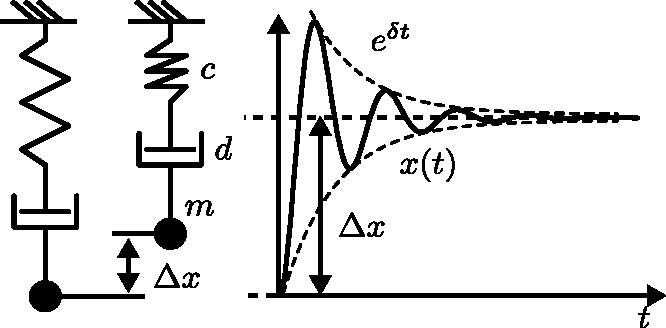
\includegraphics[width=0.65\linewidth]{Abbildungen/Modellbildung/PDF/MasseFederDaempfer.pdf}
	\caption{Feder, Masse, Dämpfer System und dessen Verhalten bei Auslenkung um eine Gleichgewichtslage}
	\label{fig:federmassedaempfer}
\end{figure}  
%
%############################################################################
\section{Beschreibung lineare Systeme im Frequenzbereich}
%############################################################################
%
%############################################################################
\subsection{Fourier Reihenentwicklung}
%############################################################################
%
Die Zerlegung von Funktionen in ihre unterschiedlichen Bestandteile und die Darstellung als Summe dieser Bestandteile sind ein gängiges Mittel, um komplizierte Funktionen zu vereinfachen. Eine Besonderheit stellen periodische Zeitfunktionen dar. Diese können durch eine Summe von unendlich vielen Sinus- und Cosinusfunktionen dargestellt werden, da diese ebenfalls periodisch sind. Diese Aussage kennen wir von den sogenannten
Fourier-Reihen \cite{Furlan08}.
%
\begin{equation}
\begin{aligned}
u(t)&=\frac{A_{0}}{2}+\sum_{k=1}^{\infty}A_{k}\cos(k\omega_{0}t)+\sum_{k=1}^{\infty}B_{k}\sin(k\omega_{0}t)
\end{aligned}
\end{equation}
%
\begin{figure}[h]
	\centering
	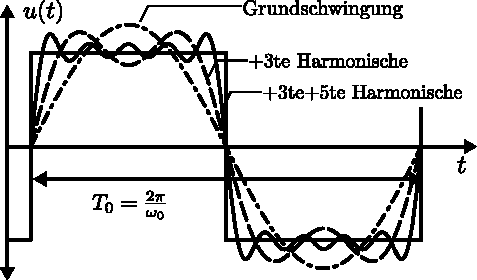
\includegraphics[width=0.675\linewidth]{Abbildungen/Modellbildung/PDF/Fourierreihe.pdf}
	\caption{Annäherung einer periodischen Rechteckfunktion mittels Fourierreihen, in Anlehnung an \cite{Lunze10}}
	\label{fig:fourierreihe}
\end{figure}  
%
Beispielsweise kann hierdurch eine periodische Rechteckfunktion $u(t)$ durch eine Summe von Sinustermen dargestellt werden (Abbildung~\ref{fig:fourierreihe}). Die Faktoren $A_{0}$,$A_{k}$ und $B_{k}$ erhält man aus den Integralbeziehungen
%
\begin{equation*}
\begin{aligned}
A_{0}&=\frac{2}{T_{0}}\int_{0}^{T_{0}}u(t)\text{d}t \quad\\
A_{k}&=\frac{2}{T_{0}}\int_{0}^{T_{0}}u(t)          \cos(k\omega_{0}t)\text{d}t \quad (k=1,2,\ldots)\\
B_{k}&=\frac{2}{T_{0}}\int_{0}^{T_{0}}u(t)\sin(k\omega_{0}t)\text{d}t \quad (k=1,2,\ldots)
\end{aligned}
\end{equation*} 
%
\begin{simulation}{}{}
	\begin{itemize}
		\item \textit{Fourierreihenentwicklung einer Sägezahnfunktion}
		\item \textit{Fourierreihenentwicklung einer Rechteckschwingung}
	\end{itemize}
\end{simulation}
%
Da die Zeitfunktionen sich in diesem Fall nur in Frequenz und Amplitude unterscheiden, können Sie auch als diskretes Frequenzspektrum dargestellt werden, ohne das Informationen verloren gehen (vgl. Abbildung~\ref{fig:spektrumdiskret}). Hieraus ergibt sich die Bezeichnung: \glqq{}im Frequenzbereich beschreiben\grqq{}. Hierbei können entweder die Amplituden der jeweiligen sinus- und cosinus-Terme in ein Diagramm eingetragen werden, oder es wird eine Darstellung aus Betrag und Phase gewählt. Im Folgenden wird die Darstellung mittels Betrag und Phase angegeben, da sie für die weitere Vorlesung wesentlich interessanter ist.
%
\begin{figure}[h]
	\centering
	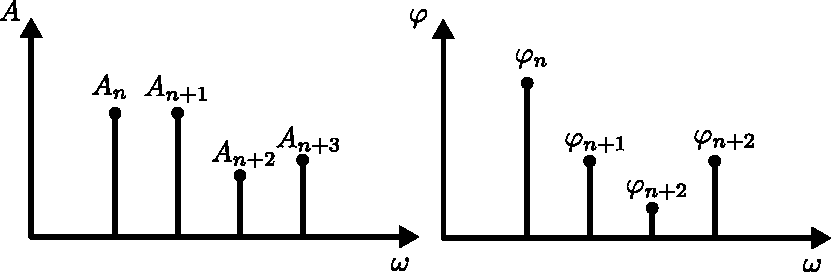
\includegraphics[width=0.75\linewidth]{Abbildungen/Modellbildung/PDF/DiskretesSpektrum.pdf}
	\caption{Darstellung der sinus- und cosinus-Funktionen der Fourierreihe mittels Betrag und Phase als diskretes Spektrum}
	\label{fig:spektrumdiskret}
\end{figure}
%
Eine kompaktere Darstellung im Gegensatz zur Schreibweise mittels getrennter sinus- und cosinus Funktionen, kann durch den Zusammenhang 
%
\begin{equation*}
\begin{aligned}
e^{-jk\omega_{0}t}&=\cos(k\omega_{0}t)-j\sin(k\omega_{0}t)
\end{aligned}
\end{equation*} 
%
erreicht werden. Die Berechnung der Koeffizienten wird durch diese Formulierung in komplexer Schreibweise dargestellt
%
\begin{equation*}
\begin{aligned}
F_{k}&=\frac{1}{T_{0}}\int_{t_{0}}^{t_{0}+T_{0}}u(t)e^{-jk\omega_{0}t}\text{d}t \quad (k=0,\pm 1,\pm 2,\ldots)
\end{aligned}
\end{equation*} 
%
muss aber nach der Berechnung noch umgewandelt werden in Betrag und Phase, was der vorherigen Darstellung in Abbildung~\ref{fig:spektrumdiskret} entspricht. 
%
%############################################################################
\subsection{Fouriertransformation}
%############################################################################
%
Werden nun nichtperiodische Funktionen betrachtet (z.B. Sprung, Impuls), welche quasi eine unendliche Periode $T_{0}$ haben, kann die Funktion nicht mehr durch diskrete Frequenzen und Phasenlagen beschrieben werden. Die einzelnen diskreten Fourierkoeffizienten bei periodischen Signalen rücken bei immer größer werdender Periode immer näher zusammen und bilden schlussendlich beim Übergang zu einer unendlichen Periode eine kontinuierliche Funktion. Diese Funktion wird auch als die Fouriertransformierte des jeweiligen Zeitsignals $u(t)$ bezeichnet und beschreibt die Frequenzanteile bezogen auf sinus- und cosinusförmige Signale.
%
\begin{equation*}
\begin{aligned}
F(j\omega)&=\int_{-\infty}^{\infty}u(t)e^{-j\omega t}\text{d}t 
\end{aligned}
\end{equation*} 
%
Neben Zeitfunktionen lassen sich auch Differentialgleichungen unter gewissen Randbedingungen mittels Fouriertransformation in eine Darstellung im Frequenzbereich transformieren. Dies ist eine der ursprünglichen Intentionen des Erfinders und wurde genutzt, um Lösungen für partielle Differentialgleichungen in der Wärmetheorie zu untersuchen. Die Fouriertransformation führt im wesentlichen dazu, dass ein Differential- in einen algebraischen Zusammenhang überführt wird. 
%
%\begin{Aufgaben}{}{}
%	\begin{itemize}
%		\item \textit{Fouriertransformation Beispiele mittels Tabelle und vollständig}
%	\end{itemize}
%\end{Aufgaben}
%
%##################################################
\subsection{Der Frequenzgang eines LZI-Übertragungsgliedes} 
%##################################################
%
%############################################################################
\subsubsection{Allgemeine Betrachtung des Frequenzgang}
%############################################################################
%
Der Frequenzgang $G(j\omega)$ eines LZI-Systems beschreibt wie sich der Systemausgang $y(t)$ auf eine Anregung mit einer Sinusfunktion am Eingang $u(t)$ verhält. 
%
\begin{figure}[h]
	\centering
	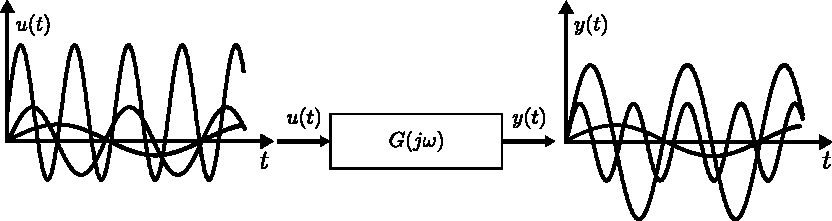
\includegraphics[width=1\linewidth]{Abbildungen/Modellbildung/PDF/Frequenzgang.pdf}
	\caption{Prinzipdarstellung des Frequenzgangs von LZI-Gliedern, in Anlehnung an \cite{Lunze10}}
	\label{fig:frequenzgang}
\end{figure}  
%
Wichtig ist zu vermerken, dass keine Anfangswerte berücksichtigt werden und das, dass Systemverhalten nur für den stationären Fall abgebildet wird (Ausgleichsvorgänge sind abgeklungen). Der Zusammenhang zur Fouriertransformierten entsteht, wenn die Berechnung aus \eqref{eq:faltung} mit sinusförmigen Eingangsfunktionen $u(t)$ berechnet wird (ohne Herleitung). Der Frequenzgang eines Systems ist somit die Fouriertransformierte der Gewichtsfunktion.
%
\begin{equation*}
\begin{aligned}
G(j\omega)&=\mathcal{F}\{g(t)\}
\end{aligned}
\end{equation*}
%
Der Frequenzgang ist in der Regelungstechnik einer der wichtigsten Werkzeuge, da er die Grundlage vieler Analysen bildet. Er lässt sich zudem messtechnisch ermitteln, da er durch Zeitfunktionen am Eingang und der Messung der Systemantworten am Ausgang bestimmt werden kann. Das Ausgangssignal ist lediglich in Amplitude und Phasenlage unterschiedlich zum Eingang, jedoch ändert sich nicht die Frequenz. In der komplexen Darstellung lässt sich der Frequenzgang wie folgt beschreiben
%
\begin{equation*}
\begin{aligned}
G(j\omega)&=\frac{Y(j\omega)}{U(j\omega)}\\
&=\frac{\hat{y}(j\omega)e^{j\omega}e^{j\varphi_{y}(j\omega)}}{\hat{u}(j\omega)e^{j\omega}e^{j\varphi_{u}}}\\
&=\frac{\hat{y}(j\omega)}{\hat{u}(j\omega)}e^{j\varphi_{yu}(j\omega)}
\end{aligned}
\end{equation*}
%
Jedoch gibt es auch die Möglichkeit den Frequenzgang in Betrag und Phase darzustellen
%
\begin{equation*}
\begin{aligned}
G(j\omega)&=\Re\{G(j\omega)\}+j\Im\{G(j\omega)\}\\
\left|G(j\omega)\right|&=\sqrt{\left(\Re\{G(j\omega)\}\right)^{2}+\left(\Im\{G(j\omega)\}\right)^{2}}\\
\angle G(j\omega)&=\arctan\left(\frac{\Im\{G(j\omega)\}}{\Re\{G(j\omega)\}}\right)
\end{aligned}
\end{equation*}
%
Zwei Darstellungen beschreiben den Frequenzgang grafisch.
%
\begin{itemize}
	\item Ortskurve, welche ein Zeigerdiagramm in der komplexen Ebene mit $\omega$ als Parameter darstellt.
	\item Bodediagramm oder Frequenzkennliniendiagramm in logarithmischer Darstellung.
\end{itemize}
%
\subsubsection{Die Ortskurve eins LZI-Übertragungsgliedes}
%
Die Ortskurve stellt den Amplituden- und Phasengang des Frequenzgangs in der komplexen Ebene mit $\omega$ als Parameter dar. Dieser Zusammenhang ist in Abbildung~\ref{fig:Ortskurve} dargestellt.
%
\begin{figure}[h!]
	\centering
	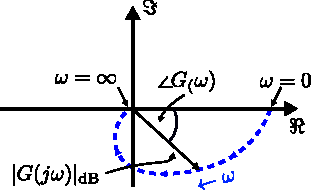
\includegraphics[width=0.45\linewidth]{Abbildungen/Modellbildung/PDF/Ortskurve.pdf}
	\caption{Ortskurve eines dynamischen System}
	\label{fig:Ortskurve}
\end{figure}
%
Über die Grenzwerte im Frequenzbereich lassen sich die Funktionen im Diagramm zeichnen. Nehmen wir das IT$_{1}$-Glied als Beispiel (aus \cite{Lunze10}), so erhalten wir für den Frequenzgang
%
\begin{equation*}
\begin{aligned}
%
G(j\omega)&=\frac{1}{j\omega T_{\text{I}}\left(j \omega T_{1}+1\right)}\\
%
&=\frac{1}{\left(-\omega^{2}T_{\text{I}}T_{1}+j\omega T_{\text{I}}\right)}\cdot\frac{\left(-\omega^{2}T_{\text{I}}T_{1}-j\omega T_{\text{I}}\right)}{\left(-\omega^{2}T_{\text{I}}T_{1}-j\omega T_{\text{I}}\right)}\\
%
&=\frac{-\omega T_{1}-j}{\omega T_{\text{I}}\left(\omega^{2}T^{2}_{1}+1\right)}\\
%
&=\frac{-T_{1}}{T_{\text{I}}\left(\omega^{2}T^{2}_{1}+1\right)}-j\frac{1}{\omega T_{\text{I}}\left(\omega^{2}T^{2}_{1}+1\right)}\\
%
\end{aligned}
\end{equation*} 
%
Hieraus lassen sich nun der Anfangs- und Endwert aus der Grenzwertbetrachtung
%
\begin{equation*}
\begin{aligned}
%
\lim\limits_{\omega\rightarrow \infty}G(j\omega)&=0\\
%
\lim\limits_{\omega\rightarrow 0}\Re\{G(j\omega)\}&=-\frac{T_{1}}{T_{\text{I}}}\\
%
\lim\limits_{\omega\rightarrow 0}\Im\{G(j\omega)\}&=-\infty.
%
\end{aligned}
\end{equation*} 
%
ermitteln und nachfolgend die Ortskurve zeichnen (siehe Abbildung~\ref{fig:OrtskurveIT1}).
%
\begin{figure}[h!]
	\centering
	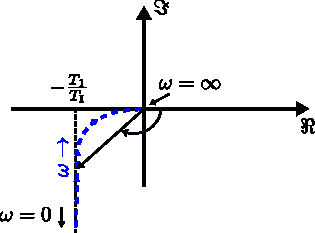
\includegraphics[width=0.50\linewidth]{Abbildungen/Systemanalyse/PDF/OrtskurveIT1.pdf}
	\caption{Ortskurve des IT$_{1}$-Gliedes}
	\label{fig:OrtskurveIT1}
\end{figure}
%
Es soll hier zudem erwähnt werden, dass der Verlauf der Amplitude und der Phase von $\omega=0$ bis $\omega=\infty$ auch durch die bekannten Verfahren der Frequenzkennlinie berechnet werden kann. 
%
\subsubsection{Die Frequenzkennlinien oder Bodediagramm eins LZI-Übertragungsgliedes \cite{Lunze10}}
%
Die Darstellung in der Ortskurve ist nicht die einzige Möglichkeit, um das Verhalten eines dynamischen Systems im Frequenzbereich zu analysieren. Allgemein wird diese auch als Frequenzkennlinie (FKL) bezeichnet. Eine sehr allgemeine, aber durchaus recht vollständige Darstellung des Frequenzgang kann durch folgende Beschreibung erreicht werden:
%
\begin{equation*}
\begin{aligned}
%
G(j\omega)=k \underbrace{\cdot \frac{1}{(j\omega)^{q}}}_{\text{I-Glieder}} \cdot \underbrace{\frac{\prod_{i=1}\left(j \omega T_{i}+1\right)}{\prod_{\nu=1}\left(j \omega T_{\nu}+1\right)}}_{\text{PT}_{1}~\text{-Glieder}} 
%
\cdot\underbrace{\frac{\prod_{k=1}\left(\left(\frac{j \omega}{\omega_{0 k}}\right)^{2}+\frac{j \omega}{\omega_{0 k}} 2 d_{k}+1\right)}{\prod_{\mu=1}\left(\left(\frac{j \omega}{\omega_{0 \mu}}\right)^{2}+\frac{j \omega}{\omega_{0 \mu}} 2 d_{\mu}+1\right)}}_{\text{PT}_{2}~\text{-Glieder}} 
%
\cdot \underbrace{e^{-T_{t}j\omega}}_{\text{Totzeit-Glied}} 
%
\end{aligned}
\end{equation*}  
%
gebracht. Durch die Überlagerung dieser Grundglieder lässt sich der Frequenzgang $G(j\omega)$ möglichst genau darstellen. Bedingung hierfür ist jedoch das:
%
\begin{itemize}
	\item $0<d_{k},d_{\mu}<1$: gedämpft aber schwingungsfähig.
	\item $\omega_{0k},\omega_{0\mu},T_{i},T_{\nu},T_{t}>0$: Kausalitätsbedingung.
	\item $k>0$: Gegenkopplungsbedingung.
	\item $q \le 2$: Bedingung für Stabilitätsnachweis über vereinfachtes Nyquistkriterium. 
\end{itemize}
%
Somit ergibt sich, dass $G(j\omega)$ sich aus den Frequenzgängen der Grundglieder und deren Inversen zusammensetzt. Die Rechenregeln hierfür lauten:
%
\begin{equation*}
\begin{aligned}
%
\quad\quad &G(j\omega)=|G(j\omega)|e^{j\varphi},\,\varphi=\angle G(j\omega)\\
%
\end{aligned}
\end{equation*}
%
Die Inversionsregel ergibt sich zu:
%
\begin{equation*}
\begin{aligned}
%
\quad\quad  &G^{-1}(j\omega)=\frac{1}{|G(j\omega)|}e^{-j\varphi}\\
%
&|G^{-1}(j\omega)|=\frac{1}{|G(j\omega)|}.\\
%
\end{aligned}
\end{equation*}
%
Was sich im Amplituden und Phasengang zu:
%
\begin{equation*}
\begin{aligned}
%
&|G^{-1}(j\omega)|_{\text{dB}}=20\lg\left(\frac{1}{|G(j\omega)|}\right)=-20\lg\left(|G(j\omega)|\right)\\
%
&\angle G^{-1}(j\omega) = - \angle G(j\omega)
%
\end{aligned}
\end{equation*}
%
ergibt. Es ist ersichtlich, dass die Inversion zu einer Spiegelung der FKL an der Null-Linie führt ($0_{\text{dB}}$ bzw. $0^{\circ}$).\\ Die Multiplikationsregel hingegen ergibt sich zu:
%
\begin{equation*}
\begin{aligned}
%
\quad\quad &G(j\omega)=G_{1}(j\omega)\cdot G_{2}(j\omega) \cdot\ldots\cdot G_{n}(j\omega)\\
%
&G(j\omega)=|G_{1}(j\omega)|e^{j\varphi_{1}}\cdot|G_{2}(j\omega)|e^{j\varphi_{2}}\cdot \ldots \cdot |G_{n}(j\omega)|e^{j\varphi_{n}}\\
%
&G(j\omega)=\left(|G_{1}(j\omega)|\cdot|G_{2}(j\omega)|\cdot\ldots\cdot|G_{n}(j\omega)\right)e^{j\left(\varphi_{1}+\varphi_{2}+\ldots+\varphi_{n}\right)}\\
%
\end{aligned}
\end{equation*}
%
Was sich im wiederum im Amplituden- bzw. Phasengang zu:
%
\begin{equation*}
\begin{aligned}
%
|G(j\omega)|_{\text{dB}}&=20\lg\left(|G_{1}(j\omega)|\cdot|G_{2}(j\omega)|\cdot\ldots\cdot|G_{n}(j\omega)\right)\\
%
&=20\lg\left(|G_{1}(j\omega)|\right)+20\lg\left(|G_{2}(j\omega)|\right)+\ldots+20\lg\left(|G_{n}(j\omega)|\right)\\
%
\angle G(j\omega) &=\angle G_{1}(j\omega)+\angle G_{2}(j\omega)+\ldots+\angle G_{n}(j\omega)
%
\end{aligned}
\end{equation*}
%
ergibt. Das bedeutet, dass eine Multiplikation der Frequenzgänge eine Addition in der FKL zur Folge hat.\\
\underline{Hinweis:} Eine Multiplikation ist gleichbedeutend mit der Hintereinanderschaltung einzelner Übertragungsglieder im Wirkschaltplan.\\
%
%Das Bodediagramm ist eine graphische Darstellung des Frequenzgang. Hierbei wird der Amplitudengang $\left|G(j\omega)\right|$ und der Phasengang $\angle G(j\omega)$ in zwei getrennte Abbildungen eingetragen. Um größere Frequenzbereiche für $\omega$ einzeichnen zu können, wird der Amplitudengang meist logarithmisch aufgetragen. Dabei gilt der Zusammenhang
%%
%\begin{equation*}
%\begin{aligned}
%\left|G(j\omega)\right|_{\text{dB}}=20 \lg \left|G(j\omega)\right|\\
%\angle G(j\omega)=\text{argmin}\left(G(j\omega)\right)
%\end{aligned}
%\end{equation*}
%
Für den Betrag und die Phase eines PT$_{1}$ Übertragungsgliedes, lassen sich folgende Berechnung schritte aufzeigen.
%
\begin{equation*}
\begin{aligned}
%
G(j\omega)&=\frac{K_{\text{P}}}{T_{1}j\omega+1}=\frac{K_{\text{P}}}{T_{1}j\omega+1}\cdot\frac{-T_{1}j\omega+1}{-T_{1}j\omega+1}=\frac{K_{\text{P}}\left(1-T_{1}j\omega\right)}{T^{2}_{1}\omega^{2}+1}\\
%
|G(j\omega)|_{\text{dB}}&=20\lg|G(j\omega)|=20\lg\left(\frac{K_{\text{p}}}{\sqrt{T^{2}_{1}\omega^{2}+1}}\right)\\
%
&=20\lg\left(K_{\text{p}}\right)-20\lg\left(\sqrt{T_{1}^{2}\omega^{2}+1}\right)\\
%
\angle G(j\omega)&=\arctan\left(\frac{-\frac{K_{\text{p}}\omega T_{1}}{T^{2}_{1}\omega^{2}+1}}{\frac{K_{\text{p}}}{T^{2}_{1}\omega^{2}+1}}\right)=\arctan\left(-\omega T_{1}\right)=-\arctan\left(\omega T_{1}\right)\\
\end{aligned}
\end{equation*}
%
\begin{figure}[ht!]
	%
	\centering
	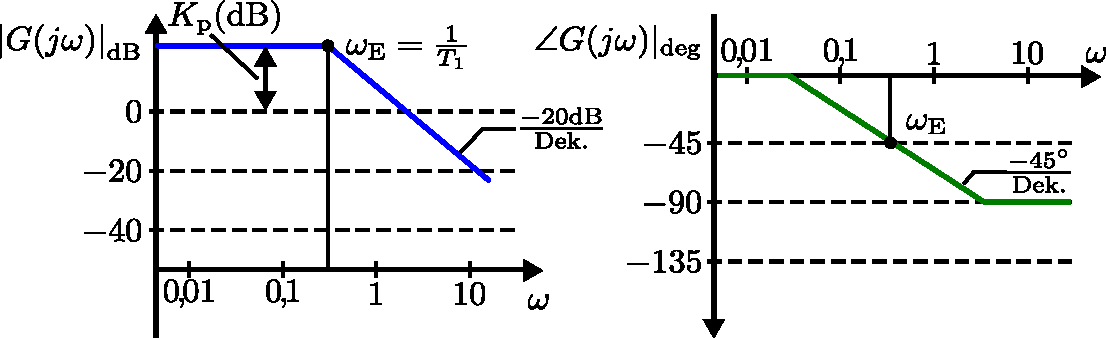
\includegraphics[width=0.9\linewidth]{Abbildungen/Modellbildung/PDF/PT1gliedBode.pdf}
	\caption{Bodediagramm zur Darstellung des Frequenzgangs, exemplarisch für ein dynamisches System}
	\label{fig:bodediagramm}
	%
\end{figure} 
%
Zur grafischen Darstellung wird auf der horizontalen Achse die Frequenz und auf der vertikalen die Amplitude aufgetragen. Die Frequenz wird meist in einer logarithmischen Skala angegeben. D.h. in linearer Unterteilung als $\lg\omega$ oder als Zehnerpotenzen mit $\omega$. 
%
Der Amplitudengang wird in Dezibel gegen die logarithmische Frequenz aufgetragen während der Phasengang unverändert auf der vertikalen Achse gegen die logarithmische Frequenz aufgetragen wird.
Es bietet sich an die beiden Diagramme bei der Konstruktion untereinander zu zeichnen und die Frequenz in gleicher Skalierung aufzutragen. Die vorgenannte Formalen Zusammenhänge sind in Abbildung~\ref{fig:bodediagramm} qualitativ dargestellt. 
%
\newpage
%############################################################################
\subsection{Laplacetransformation}
%############################################################################
%
%Der Frequenzgang ist nicht geeignet, um die Dämpfung eines technischen Systems zu beschreiben bzw. zu analysieren. Dämpfung tritt physikalisch meist durch eine Umwandlung von innerer Energie in Wärme auf. 
Die Laplacetransformation kann als Erweiterung der Fouriertransformationen verstanden werden. Diese Erweiterung ermöglicht es z.B. Differenzialgleichungen über den sogenannten Bildbereich zu lösen (vgl. Abbildung~\ref{fig:laplacetransformation}). Der Bildbereich stellt sämtliche Differentiale aus dem Zeitbereich in algebraischen Gleichungen dar.
%
\begin{figure}[h]
	\centering
	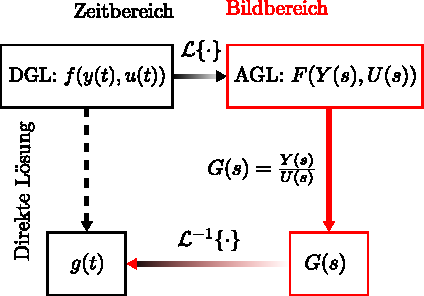
\includegraphics[width=0.55\linewidth]{Abbildungen/Modellbildung/PDF/LaplaceTransformation.pdf}
	\caption{Darstellung der Laplacetransformation zur Lösung von Differenzialgleichungen}
	\label{fig:laplacetransformation}
\end{figure}
%
Nun tritt z.B. beim Feder-Masse-Dämpfer in Abbildung~\ref{fig:federmassedaempfer} eine Dämpfung der Schwingung in Form einer Exponentialfunktion auf, die dafür sorgt, dass die sich ergebende Schwingung abklingt und das System nach einer endlichen (theoretisch unendlichen) Zeit wieder in eine Ruhelage übergeht. Dieses Verhalten, dass sogenannte Übergangsverhalten kann durch den Frequenzgang nicht abgebildet werden. Um diese Eigenschaft eines Systems jedoch trotzdem im Frequenzbereich (Bildbereich) mit all seinen Vorteilen zu erfassen, erweitert die Laplacetransformation \eqref{eq:laplace} den Frequenzbereich der Fouriertransformation um Exponentialfunktionen mit $s=\delta+j\omega$ zu
%
\begin{equation}
\begin{aligned}
F(s)&=\int_{0}^{\infty}f(t)e^{-st}\text{d}t\label{eq:laplace}
\end{aligned}
\end{equation}
%
Zudem ist zu beachten, das die Integral Grenzen nun nur von $0$ bis $\infty$ reichen, da wir annehmen, dass alle nicht periodischen Signale kausal und somit für $t<0$ nicht definiert sind. Das Hauptaugenmerk für die Behandlung in der Regelungstechnik ist, wie bereits oben erwähnt, dass sich mit Hilfe der Beziehung \eqref{eq:laplace} Differentialgleichungen nun durch algebraische Gleichungen darstellen lassen. Hierfür gibt es meist Rechentabellen, welche die wichtigsten Beziehungen zwischen Zeitbereich und Bildbereich darstellen.\\
%
Die Laplace-Transformation hat auch eine grafische Interpretation, denn sie Erweitert das kontinuierliche Spektrum der Fouriertransformation für Signale mit abklingenden e-Funktionen. 
%
%############################################################################
\subsubsection{Übertragungsfunktion}
%############################################################################
%
Die Übertragunsfunktion eines Systems ist die Laplacetransformierte der Gewichtsfunktion \eqref{eq:uebertragungsfunktion}.
%
\begin{equation}
\begin{aligned}
G(s)&=\mathcal{L}\{g(t)\}\label{eq:uebertragungsfunktion}
\end{aligned}
\end{equation}
%
Auch hier ist wieder zu erwähnen, dass keine Anfangswerte berücksichtigt werden, jedoch können Einschwingvorgänge abgebildet werden. Dies ist besonders wichtig, wenn keine sinusförmigen Eingänge auf das System wirken. Der Übergang zurück zum Frequenzgang entsteht, wenn wir eine sinusförmige Anregung an ein System anlegen und alle Einschwingvorgänge abgeklungen sind $t\rightarrow\infty$, oder wenn es im System keine Dämpfung gibt $\delta=0$. 
%
Aus diesem Grund können beide Übertragungseigenschaften zur Analyse von Regelung und Regelstrecke herangezogen werden. Auch die Übertragungsfunktion lässt sich messtechnisch ermitteln, jedoch ist dies meist schwieriger wie im Falle des Frequenzgangs und wird deshalb im späteren Verlauf der Vorlesung nur für einige Spezialfälle behandelt. Die Darstellung der Übertragungsfunktion kann folgendermaßen aussehen: 
%
\begin{equation*}
\begin{aligned}
G(s)&=\frac{Y(s)}{U(s)}\\
&=\frac{\hat{y}(s)e^{j\varphi_{y}(s)}}{\hat{u}(s)e^{j\varphi_{u}(s)}}\\
&=\frac{\hat{y}(s)}{\hat{u}(s)}e^{j\varphi_{y}(s)-\varphi_{u}(s)}
\end{aligned}
\end{equation*}
%
Jedoch gibt es auch die Möglichkeit der Übertragungsfunktion in Betrag und Phase darzustellen
%
\begin{equation*}
\begin{aligned}
G(s)&=\Re\{G(s)\}+j\Im\{G(s)\}\\
\left|G(s)\right|&=\sqrt{\left(\Re\{G(s)\}\right)^{2}+\left(\Im\{G(s)\}\right)^{2}}\\
\angle G(s)&=\arctan\left(\frac{\Im\{G(s)\}}{\Re\{G(s)\}}\right)
\end{aligned}
\end{equation*}
%
Die Übertragungsfunktion wird hauptsächlich zur Reglerauslegung verwendet.
%
\begin{itemize}
	\item Pol-Nullstellen Diagramm $\rightarrow$ Analyse der Pollage und Stabilitätsuntersuchung der offenen Wirkungskette.
	\item Wurzelortsurve $\rightarrow$ Regelerauslegung anhand der Pollage bei veränderlicher Verstärkung
\end{itemize}
%
%############################################################################
\subsubsection{Allgemeine Berechnung der Übertragungsfunktion aus der Differentialgleichung}
%############################################################################
%
Mittels der Laplacetransformation lassen sich gewöhnliche lineare Differenzialgleichungen in algebraische Gleichungen 'umwandeln'. 
\begin{itemize}
\item Schritt 1: Aufstellen der Differenzialgleichung.
%
\begin{equation*}
\begin{aligned}
a_{n}\frac{\text{d}^{n}y}{\text{d}t^{n}}+&a_{n-1}\frac{\text{d}^{n-1}y}{\text{d}t^{n-1}}+\cdots+a_{1}\frac{\text{d}y}{\text{d}t}+a_{0}y=\\
&b_{q}\frac{\text{d}^{q}u}{\text{d}t^{q}}+b_{q-1}\frac{\text{d}^{q-1}u}{\text{d}t^{q-1}}+\cdots+b_{1}\frac{\text{d}u}{\text{d}t}+b_{0}u\\
\end{aligned}
\end{equation*}
%
\item Schritt 2: Transformation in den Bildbereich durch Rechentabelle und Ableitungsregel (Anfangswerte vernachlässigen).
%
\begin{equation*}
\begin{aligned}
a_{n}s^{n}Y(s)+&a_{n-1}s^{n-1}Y(s)+\cdots+a_{1}sY(s)+a_{0}Y(s)=\\
&=b_{q}s^{q}U(s)+b_{q-1}s^{q-1}U(s)+\cdots+b_{1}sU(s)+b_{0}U(s)\\
\end{aligned}
\end{equation*}
%
\item Schritt 3: Ausklammern und umstellen
%
\begin{equation*}
\begin{aligned}
Y(s)&\left(a_{n}s^{n}+a_{n-1}s^{n-1}+\cdots+a_{1}s+a_{0}\right)=\\
&=U(s)\left(b_{q}s^{q}+b_{q-1}s^{q-1}+\cdots+b_{1}s+b_{0}\right)\\
\end{aligned}
\end{equation*}
%
%
\item Schritt 4: Übertragungsfunktion aufstellen
%
\begin{equation*}
\begin{aligned}
G(s)=\frac{b_{q}s^{q}+b_{q-1}s^{q-1}+\cdots+b_{1}s+b_{0}}{a_{n}s^{n}+a_{n-1}s^{n-1}+\cdots+a_{1}s+a_{0}}\\
\end{aligned}
\end{equation*}
%
\end{itemize}
%
%############################################################################
\subsubsection{Beispiel: Feder-Masse-Dämpfer}
%############################################################################
%
Nehmen wir zunächst die Differentialgleichung des Feder-Masse-Dämpfers ohne äußere Anregung
%
\begin{equation*}
\begin{aligned}
m\cdot \frac{\text{d}^{2}x(t)}{\text{d}t^{2}} + d\cdot \frac{\text{d}x(t)}{\text{d}t} + c x(t)=0
\end{aligned}
\end{equation*}
%
so ließe sich durch Anwendung der Laplacetransformation folgender Zusammenhang finden
%
\begin{equation*}
\begin{aligned}
\underbrace{s^{2}X(s)-sx(0)-\frac{\text{d}x(0)}{\text{d}t}}_{s^{2}\mathcal{L}\{f(t)\}-sf(0)-\frac{\text{d}f(0)}{\text{d}t}} + \underbrace{\frac{d}{m}\left(sX(s)-x(0)\right)}_{s\mathcal{L}\{f(t)\}-f(0)} + \frac{c}{m}X(s)=0
\end{aligned}
\end{equation*}
%
Da Anfangswerte vernachlässigt werden, können wir die Gleichung umwandeln in
%
\begin{equation*}
\begin{aligned}
s^{2}X(s) + \frac{d}{m}X(s)s + \frac{c}{m}X(s)=0
\end{aligned}
\end{equation*}
%
Durch Umstellen der Gleichung erhalten wir nun die Übertragungsfunktion des Systems im Laplace Bereich
%
\begin{equation*}
\begin{aligned}
G(s)= \frac{1}{s^{2} + \frac{d}{m}s + \frac{c}{m}}\\
%
\end{aligned}
\end{equation*}
%
Und die Übergangsfunktion durch hinzufügen eines Einheitssprung am Eingang  
%
\begin{equation*}
\begin{aligned}
%
H(s)= \frac{1}{s\left(s^{2} + \frac{d}{m}s + \frac{c}{m}\right)}
%
\end{aligned}
\end{equation*}
%
Abbildung~\ref{fig:federmassedaempfer} stellt die Sprungantwort $h(t)$ des schwingungsfähigen Systems dar. Die Anregung erfolgt in diesem Fall durch eine Auslenkung um die Ruhelage.
%
%############################################################################
\subsection{Pole und Nullstellen der Übertragungsfunktion}
%############################################################################
%
Der Pol- Nullstellenplan ermöglicht die Eigenschaften der Regelstrecke graphisch zu analysieren. Um die Pole und Nullstellen auszurechnen, müssen die Polynome der Übertragungsfunktion 
%
\begin{equation*}
\begin{aligned}
G(s)=\frac{b_{q}s^{q}+b_{q-1}s^{q-1}+\cdots+b_{1}s+b_{0}}{a_{n}s^{n}+a_{n-1}s^{n-1}+\cdots+a_{1}s+a_{0}}\\
\end{aligned}
\end{equation*}
%
in ihre einzelnen Bestandteile zerlegt werden.
%
\begin{equation}
\begin{aligned}
G(s)=k\frac{\left(s-s_{\text{N},1}\right)\left(s-s_{\text{N},2}\right)\ldots\left(s-s_{\text{N},q}\right)}{\left(s-s_{\text{P},1}\right)\left(s-s_{\text{P},2}\right)\ldots\left(s-s_{\text{P},n}\right)}=k\frac{\prod_{i=1}^{q}\left(s-s_{\text{N},i}\right)}{\prod_{i=1}^{n}\left(s-s_{\text{P},i}\right)}\label{eq:polnullstellenform}\\
\end{aligned}
\end{equation}
%
Jeder dieser Pole und Nullstellen, welche Beispielsweise durch Partialbruchzerlegung errechnet wurden, kann nun in das Pol- Nullstellendiagramm Abbildung~\ref{fig:polnullstellen} eingetragen werden.
%
\begin{figure}[h]
	\centering
	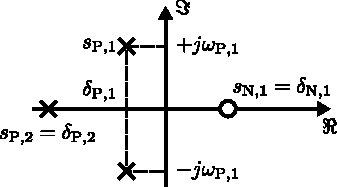
\includegraphics[width=0.48\linewidth]{Abbildungen/Modellbildung/PDF/PolNullstellen.pdf}
	\caption{Pol- Nullstellen Diagramm gebildet aus einer Übertragungsfunktion}
	\label{fig:polnullstellen}
\end{figure}
%
Wie in Abbildung~\ref{fig:polnullstellen} zu erkennen können Pole und Nullstellen sowohl reell als auch konjugiert komplex sein. Aus diesem Diagramm lassen sich jetzt direkt die zeitlichen Eigenschaften eines Systems ablesen.
%
\begin{itemize}
	\item \textbf{Dynamisches Verhalten}: 
		\begin{itemize}
			\item Sind die Pole reell ($s=\delta,\, j\omega = 0$)?
			\item Oder konjugiert komplex mit Dämpfung ($s=\delta\pm j\omega$)?
			\item Oder konjugiert komplex ohne Dämpfung ($s=\pm j\omega$)?
			\item Wie nahe sind sie der Imaginären Achse?
		\end{itemize}
		%
	\item \textbf{Stabilität}: 
		\begin{itemize}
			\item Sind alle Pole links der Imaginären Achse?
		\end{itemize}
\end{itemize}
%
\begin{Aufgaben}{}{}
	\begin{itemize}
		\item \textit{Einige Beispiele von Pol- Nullstellen Diagrammen und zugehörigen Zeitverläufen}
	\end{itemize}
\end{Aufgaben}
%
%###########################################################################
\subsubsection{Berechnung der Sprungantwort aus der Übertragungsfunktion}
%############################################################################
%
Es stellt sich die Frage, wie die Sprungantwort eines Systems nun aus der Übertragungsfunktion berechnet werden kann und welche Vorteile dies bietet. Berechnen wir mittels Partialbruchzerlegung aus der Multiplikation von \eqref{eq:polnullstellenform} und einem sprungförmigen Eingangssignal $U(s)$ nun die einzelnen Pole, ergibt sich folgende Gleichung
%
\begin{equation}
\begin{aligned}
Y(s)=G(s)U(s)=\frac{k_{0}}{s}+\frac{k_{1}}{\left(s-s_{\text{P},1}\right)}+\frac{k_{2}}{\left(s-s_{\text{P},2}\right)}+\ldots+\frac{k_{n}}{\left(s-s_{\text{P},n}\right)},\, k_{0}=\frac{b_{q}}{c_{p}}\label{eq:partialbrueche}\\
\end{aligned}
\end{equation}
%
Diese einzelnen Terme lassen sich mittels Laplace Rücktransformation nun in den Zeitbereich zurück übersetzen. Da wir in dieser Vorlesung lediglich LZI-Systeme betrachten, können die Einzelterme sowohl im Bild- als auch im Zeitbereich linear überlagert werden. Die Sprungantwort im Zeitbereich aus \eqref{eq:partialbrueche} ergibt sich zu 
%
\begin{equation}
\begin{aligned}
y(t)=h(t)=g(t)*u(t)=k_{0}+k_{1}e^{s_{\text{P},1}t}+k_{2}e^{s_{\text{P},2}t}+\ldots+k_{n}e^{s_{\text{P},n}t}\label{eq:sprungantwortlaplace}\\
\end{aligned}
\end{equation}
%
Diese Formulierung gilt nur für reellwertige Pole. Tauchen konjugiert komplexe Pole auf und sollen diese reellwertig dargestellt werden, so muss die Darstellung \eqref{eq:sprungantwortlaplace} erweitert werden, zu
%
\begin{equation*}
\begin{aligned}
%
Y(s)=G(s)U(s)=\frac{k_{1}}{\left(s-s_{\text{P},1}\right)}+\frac{k_{2}}{\left(s-s_{\text{P},2}\right)}\\
\text{mit}\,\, s_{\text{P},12}=\delta_{12}\pm j\omega_{12},\,\,k_{12}=\alpha_{12}\pm j\beta_{12}
%
\end{aligned}
\end{equation*}
%
Ausmultiplizieren und mittels eines Ansatzes lösen
%
\begin{equation*}
\begin{aligned}
%
Y(s)=G(s)U(s)=\frac{k_{1}\left(s-s_{\text{P},1}\right)+k_{2}\left(s-s_{\text{P},1}\right)}{\left(s-s_{\text{P},1}\right)\left(s-s_{\text{P},2}\right)}=\ldots=\frac{B_{1}s+B_{0}}{s^{2}+A_{1}s+A_{0}}
%
\end{aligned}
\end{equation*}
%
Durch Koeffizientenvergleich erhält man nun die reellen Koeffizienten 
%
\begin{equation*}
\begin{aligned}
%
B_{0}&=-2\left(\delta_{12}\alpha_{12}+\omega_{12}\beta_{12}\right)\\
B_{1}&=2\alpha_{12}\\
A_{0}&=\delta^{2}_{12}+\omega^{2}_{12}\\
A_{1}&=-2\delta_{12}
%
\end{aligned}
\end{equation*}
%
Diese Darstellung ist für die Rücktransformation günstiger da sie nur reelle Koeffizienten enthält und direkt über die Korrespondenztabelle abgelesen werden kann.
%
\newpage
%
%##################################################
\subsection{Lineare Grundglieder zur Beschreibung dynamischer Verhalten}
%##################################################
%
Im folgenden werden die wichtigsten linearen Grundglieder, welche für die Regelungstechnik Bedeutung haben vorgestellt. Die Inhalte dieses Kapitels können in \cite{Foellinger94, Unbehauen08, MSF05, Lunze10} nachgelesen werden.
%
%%##################################################
%\subsubsection{Proportionalglied (P-Glied)}
%%##################################################
%%
%Das Proportionalglied kennzeichnet sich durch einen konstanten Verstärkungsfaktor $K_{\text{p}}$ aus. Dieser ist aufgrund der Eigenschaften der Laplace Transformation im Zeit und im Bildbereich identisch.
%%
%\begin{itemize}
%%
%\item Funktionalbeziehung im Zeitbreich
%%
%\begin{equation*}
%\begin{aligned}
%%
%y(t)=K_{\text{p}}u(t)
%%
%\end{aligned}
%\end{equation*}
%%
%\item Laplacetransformierte und Übergangsfunktion im Bildbereich
%%
%\begin{equation*}
%\begin{aligned}
%%
%Y(s)=K_{\text{p}}U(s),\quad G(s)=K_{\text{p}},\quad H(s)=\frac{K_{\text{p}}}{s}
%%
%\end{aligned}
%\end{equation*}
%%
%\item Sprungantwort im Zeitbereich
%%
%\begin{figure}[h]
%	\centering
%	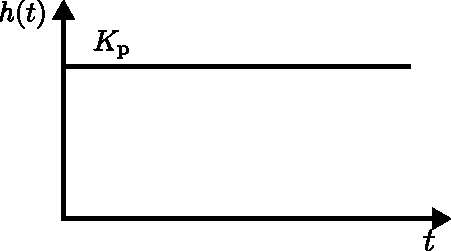
\includegraphics[width=0.375\linewidth]{Abbildungen/Modellbildung/PDF/PgliedSprung.pdf}
%	\caption{Qualitative Sprungantwort des Proportionalgliedes}
%	\label{fig:pgliedsprung}
%\end{figure}
%%
%\item Frequenzgang
%%
%\begin{equation*}
%\begin{aligned}
%%
%G(j\omega)=K_{\text{p}}
%%
%\end{aligned}
%\end{equation*}
%%
%\item Bodediagramm: Wird beim P-Glied vernachlässigt, da einfach.
%%
%\item Symbol bzw. Blockschaltbild
%%
%\begin{figure}[h]
%	\centering
%	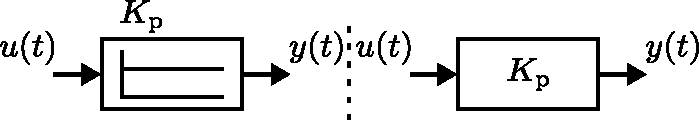
\includegraphics[width=0.65\linewidth]{Abbildungen/Modellbildung/PDF/PgliedBlock.pdf}
%	\caption{Symbol, Blockschaltbild des Proportionalgliedes}
%	\label{fig:pglied}
%\end{figure}
%%
%\end{itemize}
%%
%##################################################
\subsubsection{Integratorglied (I-Glied)}
%##################################################
%
Das I-Glied integriert den Eingang fortlaufend auf. $K_{\text{I}}=\frac{1}{T_{\text{I}}}$ stellt den Integrationsbeiwert dar. Dieser ist aufgrund der Eigenschaften der Laplace Transformation im Zeit und im Bildbereich identisch.
%
\begin{itemize}
	%
	\item Funktionalbeziehung und Darstellung im Zeitbreich
	%
	\begin{equation*}
	\begin{aligned}
	%
	y(t)=K_{\text{I}}\int_{0}^{t}u(\tau)\text{d}\tau \,\,\text{oder}\,\, y(t)=\frac{1}{T_{\text{I}}}\int_{0}^{t}u(\tau)\text{d}\tau
	%
	\end{aligned}
	\end{equation*}
	%
	\item Laplacetransformierte und Übergangsfunktion im Bildbereich
	%
	\begin{equation*}
	\begin{aligned}
	%
	Y(s)=\frac{K_{\text{I}}U(s)}{s},\quad G(s)=\frac{K_{\text{I}}}{s},\quad H(s)=\frac{K_{\text{I}}}{s^{2}}
	%
	\end{aligned}
	\end{equation*}
	%
	\item Pol- Nullstellen Diagramm im Bildbereich in Abbildung~\ref{fig:igliedpn}: Eine Polstelle im Ursprung vorhanden, zwar keinen negativen Realteil, aber definitionsgemäß instabil. 
	%
	\begin{figure}[h]
		\centering
		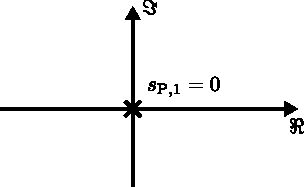
\includegraphics[width=0.4\linewidth]{Abbildungen/Modellbildung/PDF/Igliedpn.pdf}
		\caption{Qualitatives Pol- Nullstellen Diagramm des Integratorgliedes}
		\label{fig:igliedpn}
	\end{figure}
	%
	\item Sprungantwort im Zeitbereich: Ergibt sich aus der Rücktransformation von \\$H(s) \,\Laplace\, h(t)=K_{\text{I}}t$
	%
	\begin{figure}[h]
		\centering
		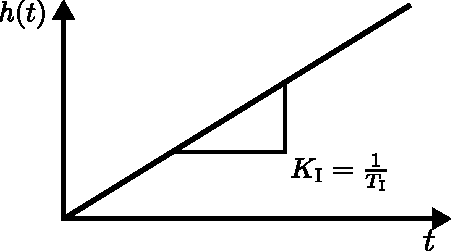
\includegraphics[width=0.375\linewidth]{Abbildungen/Modellbildung/PDF/IgliedSprung.pdf}
		\caption{Qualitative Sprungantwort des Integratorgliedes}
		\label{fig:igliedsprung}
	\end{figure}
	%
	\item Frequenzgang, Amplitudengang, Phasengang
	%
	\begin{equation*}
	\begin{aligned}
	%
	G(j\omega)&=\frac{K_{\text{I}}}{j\omega}= -j\frac{K_{\text{I}}}{\omega}\\
	%
	|G(j\omega)|_{\text{dB}}&=20\lg|G(j\omega)|=20\lg\left(\frac{K_{\text{I}}}{\omega}\right)\\
	%
	&=20\lg\left(K_{\text{I}}\right)-20\lg\left(\omega\right)\\
	%
	\angle G(j\omega)&=\arctan\left(\frac{-\frac{K_{\text{I}}}{\omega}}{0}\right)=-90^{\circ}\\
	\end{aligned}
	\end{equation*}
	%
	\item Bodediagramm in Abbildung~\ref{fig:igliedbode}: Die Durchtrittskreisfrequenz $\omega_{\text{D}}$ markiert den Punkt bei der die Verstärkung gleich $1$ oder $0$ dB ist. Der Amplitudengang kennzeichnet sich durch eine negative Steigung von $\frac{-20\text{dB}}{Dek.}$. Da der Phasengang sich nur aus negativen komplexen Anteilen zusammensetzt ist die Phase von Anfang an $-90^{\circ}$.\\\\
	%
	\begin{figure}[h]
		\centering
		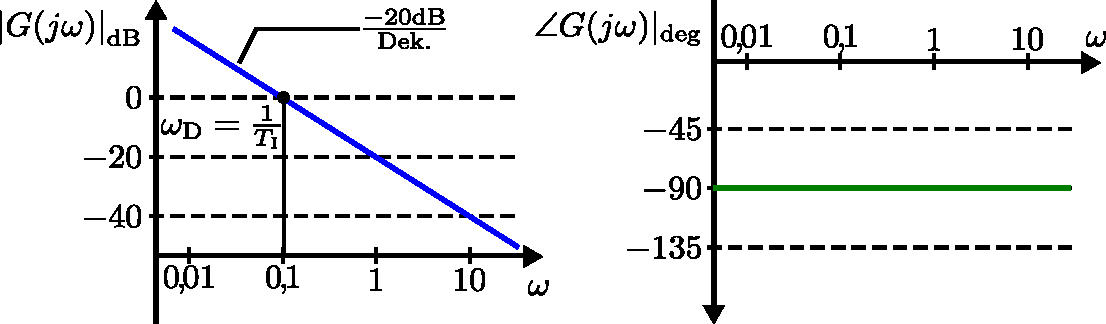
\includegraphics[width=0.85\linewidth]{Abbildungen/Modellbildung/PDF/IgliedBode.pdf}
		\caption{Qualitatives Bodediagramm des Integratorglieds}
		\label{fig:igliedbode}
	\end{figure}
	%
	\item Symbol bzw. Blockschaltbild in Abbildung~\ref{fig:igliedblock}
	%
	\begin{figure}[h]
		\centering
		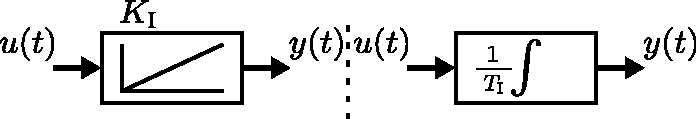
\includegraphics[width=0.625\linewidth]{Abbildungen/Modellbildung/PDF/IgliedBlock.pdf}
		\caption{Symbol, Blockschaltbild des Integratorglieds}
		\label{fig:igliedblock}
	\end{figure}
%
\end{itemize}
%
%##################################################
\subsubsection{Differenzierglied (D-Glied)}
%##################################################
%
Das Differenzierglied leitet den Eingang $u(t)$ kontinuierlich ab. Zudem exitiert ein Verstärkungsfaktor $K_{\text{D}}$. Dieser ist aufgrund der Eigenschaften der Laplace Transformation im Zeit und im Bildbereich identisch.
%
\begin{itemize}
	%
	\item Funktionalbeziehung und Darstellung im Zeitbreich
	%
	\begin{equation*}
	\begin{aligned}
	%
	y(t)=K_{\text{D}}\frac{\text{d}u(t)}{\text{d}t}
	%
	\end{aligned}
	\end{equation*}
	%
	\item Laplacetransformierte und Übergangsfunktion im Bildbereich
	%
	\begin{equation*}
	\begin{aligned}
	%
 	Y(s)=K_{\text{D}}U(s)s,\quad G(s)=K_{\text{D}}s,\quad H(s)=K_{\text{D}}
	%
	\end{aligned}
	\end{equation*}
	%
	\item Pol- Nullstellen Diagramm im Bildbereich in Abbildung~\ref{fig:dgliedpn}: Differenzierglied besitzt eine Nullstelle im Ursprung. Das System ist je nach Definition stabil; Zustandsstabil da kein Pol in der rechten Halbebene, jedoch nicht E/A-stabil, da auch Sprungstellen des Eingangssignals abgeleitet werden. Somit können unbegrenzte Ableitungen auftreten (theoretisch).
	%
	\begin{figure}[h]
		\centering
		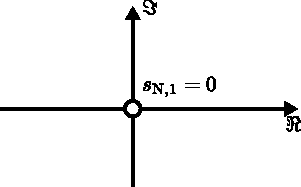
\includegraphics[width=0.4\linewidth]{Abbildungen/Modellbildung/PDF/Dgliedpn.pdf}
		\caption{Qualitatives Pol- Nullstellen Diagramm des Diffenzierglieds}
		\label{fig:dgliedpn}
	\end{figure}
	%
	%
	\item Sprungantwort im Zeitbereich: Ergibt sich aus der Rücktransformation von \\$H(s) \,\Laplace\, h(t)=K_{\text{D}}\delta(t)$. Eigenschaft des Dirac-Impuls
	%
	\begin{equation*}
	\begin{aligned}
	%
	\int_{-\infty}^{\infty}h(\tau)\text{d}\tau=K_{\text{D}}
	%
	\end{aligned}
	\end{equation*}
	%
	Ist ein Rechteck mit der Fläche $K_{\text{D}}$, welches infinitisimal schmal ist.
	%
	\item Frequenzgang, Amplitudengang, Phasengang
	%
	\begin{equation*}
	\begin{aligned}
	%
	G(j\omega)&=K_{\text{D}}j\omega\\
	%
	|G(j\omega)|_{\text{dB}}&=20\lg|G(j\omega)|=20\lg\left(K_{\text{D}}\omega\right)=20\lg\left(K_{\text{D}}\right)+20\lg\left(\omega\right)\\
	%
	\angle G(j\omega)&=\arctan\left(\frac{K_{\text{D}}\omega}{0}\right)=+90^{\circ}\\
	\end{aligned}
	\end{equation*}
	%
	\item Bodediagramm: Die Durchtrittskreisfrequenz $\omega_{\text{D}}$ markiert den Punkt bei der die Verstärkung gleich $1$ oder $0$ dB ist. Der Amplitudengang kennzeichnet sich durch eine positive Steigung von $\frac{+20\text{dB}}{Dek.}$. Da der Phasengang sich nur aus positiven komplexen Anteilen zusammensetzt ist die Phase von Anfang an $+90^{\circ}$.
	%
	\begin{figure}[h]
		\centering
		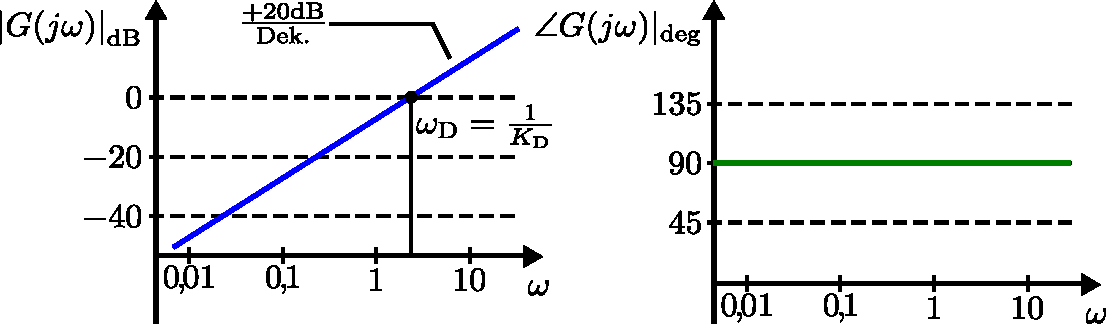
\includegraphics[width=0.8\linewidth]{Abbildungen/Modellbildung/PDF/DgliedBode.pdf}
		\caption{Qualitatives Bodediagramm des Differenzierglied}
		\label{fig:dgliedbode}
	\end{figure}
	%
	\item Symbol bzw. Blockschaltbild
	%
	\begin{figure}[h]
		\centering
		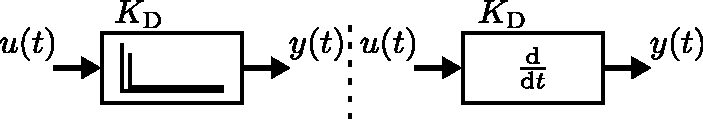
\includegraphics[width=0.65\linewidth]{Abbildungen/Modellbildung/PDF/DgliedBlock.pdf}
		\caption{Symbol, Blockschaltbild des Differenzierglied}
		\label{fig:dglied}
	\end{figure}
	%
\end{itemize}
%
%##################################################
\subsubsection{Totzeitglied (T$_{\boldsymbol{t}}$-Glied)}
%##################################################
%
Das Totzeitglied, zeichnet sich durch eine durch eine Verschiebungsfunktion aus, welche eine beliebige Zeitfunktion um einen konstanten Wert $T_{t}$ nach rechts verschiebt.
%
\begin{itemize}
	%
	\item Funktionalbeziehung
	%
	\begin{equation*}
	\begin{aligned}
	%
	y(t)=u(t-T_{t})
	%
	\end{aligned}
	\end{equation*}
	%
	\item Laplacetransformierte und Übergangsfunktion im Bildbereich
	%
	\begin{equation*}
	\begin{aligned}
	%
	Y(s)=e^{-T_{t}s}U(s),\quad G(s)=e^{-T_{t}s},\quad H(s)=\frac{e^{-T_{t}s}}{s}
	%
	\end{aligned}
	\end{equation*}
	%
	\item Pol- Nullstellen Diagramm im Bildbereich: Das Totzeitglied hat kein eigenes Diagramm, da es keine Pole oder Nullstellen besitzt.
	%
	\item Sprungantwort im Zeitbereich in Abbildung~\ref{fig:tgliedsprung}: Ergibt sich aus der Rücktransformation von \\$H(s) \,\Laplace\, h(t)=\sigma(t-T_{t})$.
	%
	\begin{figure}[h]
		\centering
		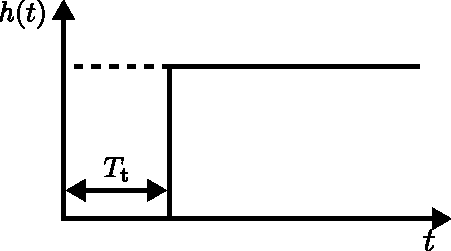
\includegraphics[width=0.4\linewidth]{Abbildungen/Modellbildung/PDF/TgliedSprung.pdf}
		\caption{Qualitative Sprungantwort des Totzeitgliedes}
		\label{fig:tgliedsprung}
	\end{figure}
	%
	\item Frequenzgang, Amplitudengang, Phasengang
	%
	\begin{equation*}
	\begin{aligned}
	%
	G(j\omega)&=e^{-T_{t}j\omega}=\cos(\omega T_{t})-j\sin(\omega T_{t})\\
	%
	|G(j\omega)|_{\text{dB}}&=20\lg|G(j\omega)|=20\lg\left(\underbrace{\sqrt{\cos^{2}(\omega T_{t})+\sin^{2}(\omega T_{t})}}_{=1}\right)=0\\
	%
	\angle G(j\omega)&=\arctan\left(\frac{-\sin(\omega T_{t})}{\cos(\omega T_{t})}\right)=-\omega T_{t}\\
	\end{aligned}
	\end{equation*}
	%
	\item Bodediagramm in Abbildung~\ref{fig:tgliedbode}: Der Amplitudengang des Totzeitgliedes ist eine konstante Linie mit der Verstärkung 1 in dB. Der Phasengang auf der anderen Seite ergibt sich als eine stark abfallende Funktion der Kreisfrequenz $\omega$. Der Phasengang hat bei $\omega=\frac{1}{T_{t}}$ eine Phase von $-57^{\circ}$.
	%
	\begin{figure}[h]
		\centering
		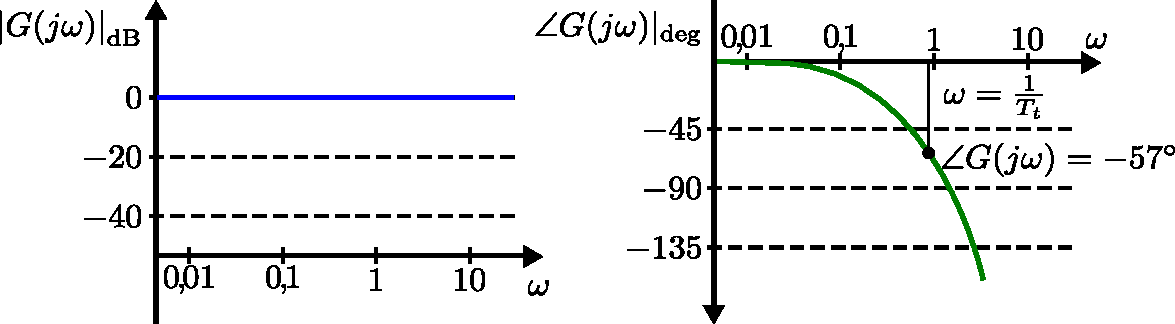
\includegraphics[width=0.9\linewidth]{Abbildungen/Modellbildung/PDF/TgliedBode.pdf}
		\caption{Qualitatives Bodediagramm des Totzeitgliedes}
		\label{fig:tgliedbode}
	\end{figure}
	%
	\item Symbol bzw. Blockschaltbild
	%
	\begin{figure}[h]
		\centering
		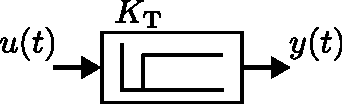
\includegraphics[width=0.3\linewidth]{Abbildungen/Modellbildung/PDF/TgliedBlock.pdf}
		\caption{Symbol, Blockschaltbild des Totzeitgliedes}
		\label{fig:tglied}
	\end{figure}
	%
\end{itemize}
%
%##################################################
\subsubsection{Verzögerungsglied 1-Ordnung (PT$_{\boldsymbol{1}}$-Glied)}
%##################################################
%
Das Verzögerungsglied erster Ordnung beschreibt ein dynamisches Verhalten wie es bei einer Differentialgleichung erster Ordnung vorkommt. Die Beiden beschreibenden Variablen ist die Zeitkonstante $T_{1}$ und der Verstärkungsfaktor $K_{\text{p}}$.
%
\begin{itemize}
	%
	\item Funktionalbeziehung im Zeitbereich
	%
	\begin{equation*}
	\begin{aligned}
	%
	T_{1}\frac{\text{d}y(t)}{\text{d}}+y(t)=K_{\text{p}}u(t)
	%
	\end{aligned}
	\end{equation*}
	%
	\item Laplacetransformierte, Übertragungsfunktion und Übergangsfunktion im Bildbereich
	%
	\begin{equation*}
	\begin{aligned}
	%
	Y(s)=\frac{K_{\text{p}}}{T_{1}s+1}U(s),\quad G(s)=\frac{K_{\text{p}}}{T_{1}s+1},\quad H(s)=\frac{K_{\text{p}}}{s\left(T_{1}s+1\right)}
	%
	\end{aligned}
	\end{equation*}
	%
	\item Pol- Nullstellen Diagramm im Bildbereich in Abbildung~\ref{fig:pt1gliedpn}: Das $\text{PT}_{1}-\text{Glied}$ besitzt eine Polstellen in der negativen Halbebene bei $s_{\text{P},1}=-\frac{1}{T_{1}}$ und keine Nullstelle. Da technische Systeme immer eine Positive (physikalische) Zeitkonstante besitzen ist diese Glied zunächst einmal stabil.
	%
	\begin{figure}[h]
		\centering
		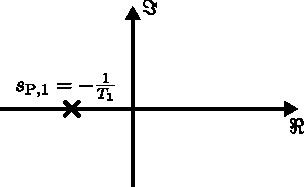
\includegraphics[width=0.4\linewidth]{Abbildungen/Modellbildung/PDF/PT1gliedpn.pdf}
		\caption{Qualitatives Pol- Nullstellen Diagramm des Verzögerungsgliedes 1-Ordnung}
		\label{fig:pt1gliedpn}
	\end{figure}
	%
	%
	\item Sprungantwort im Zeitbereich in Abbildung~\ref{fig:pt1gliedsprung}: Ergibt sich aus der Rücktransformation von $H(s) \,\Laplace\, h(t)=K_{\text{p}}\left(1-e^{-\frac{t}{T_{1}}}\right)$. Sowohl $K_{\text{p}}$ als auch $T_{1}$ lassen sich aus der Sprungantwort ermitteln.
	%
	\begin{figure}[h]
		\centering
		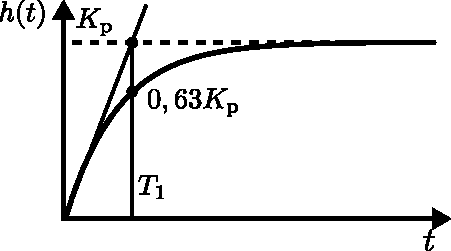
\includegraphics[width=0.4\linewidth]{Abbildungen/Modellbildung/PDF/PT1gliedSprung.pdf}
		\caption{Qualitative Sprungantwort des Verzögerungsglied 1-Ordnung}
		\label{fig:pt1gliedsprung}
	\end{figure}
	%
	\item Frequenzgang, Amplitudengang, Phasengang
	%
	\begin{equation*}
	\begin{aligned}
	%
		G(j\omega)&=\frac{K_{\text{P}}}{T_{1}j\omega+1}=\frac{K_{\text{P}}}{T_{1}j\omega+1}\cdot\frac{-T_{1}j\omega+1}{-T_{1}j\omega+1}=\frac{K_{\text{P}}\left(1-T_{1}j\omega\right)}{T^{2}_{1}\omega^{2}+1}\\
	%
	|G(j\omega)|_{\text{dB}}&=20\lg|G(j\omega)|=20\lg\left(\frac{K_{\text{p}}}{\sqrt{T^{2}_{1}\omega^{2}+1}}\right)\\
	%
	&=20\lg\left(K_{\text{p}}\right)-20\lg\left(\sqrt{T_{1}^{2}\omega^{2}+1}\right)\\
	%
	\angle G(j\omega)&=\arctan\left(\frac{-\frac{K_{\text{p}}\omega T_{1}}{T^{2}_{1}\omega^{2}+1}}{\frac{K_{\text{p}}}{T^{2}_{1}\omega^{2}+1}}\right)=\arctan\left(-\omega T_{1}\right)=-\arctan\left(\omega T_{1}\right)\\
	\end{aligned}
	\end{equation*}
	%
	\item Bodediagramm in Abbildung~\ref{fig:pt1gliedbode}: Bis zum erreichen der Knickfrequenz $\omega_{\text{E}}$ verläuft der Amplitudengang Frequenz unabhängig mit der Verstärkung $K_{\text{p}}$ in dB. Durch die Vergrößerung der Frequenz $\omega$ wird nun auch der zweite (frequenzabhängige) Term des Amplitudengangs relevant und er neigt sich bis zu einer negativen Steigung von $\frac{-20\text{dB}}{\text{Dek.}}$. Der Phasengang verhält sich zunächst auch konstant und nimmt den Wert $0^{\circ}$ an. Er fällt auf einen Wert von $-90^{\circ}$ für $\omega\rightarrow\infty$. In Höhe der Knickfrequenz $\omega_{\text{E}}$ ist die Phase $-45^{\circ}$.
	%
	\begin{figure}[h]
		\centering
		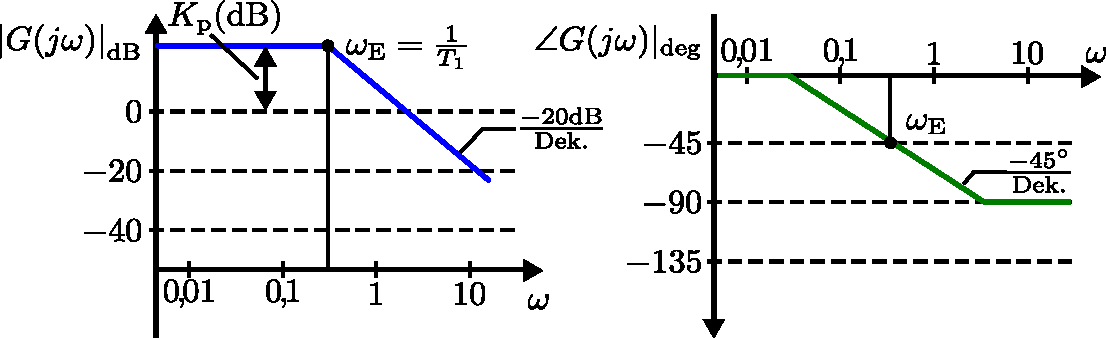
\includegraphics[width=0.9\linewidth]{Abbildungen/Modellbildung/PDF/PT1gliedBode.pdf}
		\caption{Qualitatives Bodediagramm des Verzögerungsglied 1-Ordnung}
		\label{fig:pt1gliedbode}
	\end{figure}
	%
	\item Symbol bzw. Blockschaltbild
	%
	\begin{figure}[h]
		\centering
		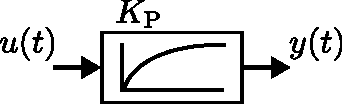
\includegraphics[width=0.3\linewidth]{Abbildungen/Modellbildung/PDF/PT1gliedBlock.pdf}
		\caption{Symbol, Blockschaltbild des Verzögerungsglied 1-Ordnung}
		\label{fig:pt1glied}
	\end{figure}
	%
\end{itemize}
%
%##################################################
\subsubsection{Verzögerungsglied 2ter-Ordnung (PT$_{\boldsymbol{2}}$-Glied)}
%##################################################
%
Das Verzögerungsglied zweiter Ordnung kann genutzt werden, um dynamische Systeme darzustellen, welche durch eine lineare Differentialgleichung 2ter-Ordnung ausgedrückt werden können (z.B. elektrischer Schwingkreis oder Kette von RC-Gliedern).
%
\begin{itemize}
	%
	\item Funktionalbeziehung im Zeitbereich
	%
	\begin{equation*}
	\begin{aligned}
	%
	T^{2}\frac{\text{d}^{2}y(t)}{\text{d}t^{2}}+2dT\frac{\text{d}y(t)}{\text{d}t}+y(t)=K_{\text{p}}u(t)
	%
	\end{aligned}
	\end{equation*}
	%
	Laplacetransformierte und Übergangsfunktion im Bildbereich
	%
	\begin{equation*}
	\begin{aligned}
	%
	Y(s)=\frac{K_{\text{p}}}{T^{2}s^{2}+2dTs+1}U(s),\quad G(s)=\frac{K_{\text{p}}}{T^{2}s^{2}+2dTs+1}\\ H(s)=\frac{K_{\text{p}}}{s\left(T^{2}s^{2}+2dTs+1\right)}
	%
	\end{aligned}
	\end{equation*}
	%
	Die Übertragungsfunktion lässt sich durch Umformung folgendermaßen darstellen
	%
	\begin{equation*}
	\begin{aligned}
	%
	G(s)&=\frac{K_{\text{p}}}{T^{2}s^{2}+2dTs+1}\\
	%
	&=\frac{K_{\text{p}}}{\frac{1}{\omega^{2}_{0}}s^{2}+\frac{2d}{\omega_{0}}s+1}, \quad \omega_{0} = \frac{1}{T}\\
	%
	&=\frac{K_{\text{p}}\omega^{2}_{0}}{s^{2}+2d\omega_{0}s+\omega^{2}_{0}}
	%
	\end{aligned}
	\end{equation*}
	%
	Und die Pole nach folgender Vorschrift berechnen
	%
	\begin{equation*}
	\begin{aligned}
	%
	&s^{2}+2d\omega_{0}s+\omega^{2}_{0}=0\\
	%
	&s_{\text{P},12}=-d\omega_{0}\pm\sqrt{d^{2}\omega^{2}_{0}-\omega^{2}_{0}}\\
	%
	&s_{\text{P},12}=-d\omega_{0}\pm\omega_{0}\sqrt{d^{2}-1}\\
	%
	\end{aligned}
	\end{equation*}
	%
	\item Pol- Nullstellen Diagramm im Bildbereich in Abbildung~\ref{fig:pt2gliedpn}: Das $\text{PT}_{2}-\text{Glied}$ hat, je nachdem welche Dämpfung $d$ das System besitzt, unterschiedliche Pole und keine Nullstelle. In Abbildung~\ref{fig:pt2gliedpn} sind die beiden Fälle für $d<1$ (konjugiert komplexe Polpaar) und $d=1$ (doppelter Reeller Pol) dargestellt. Für $d>1$ ergeben sich zwei unterschiedliche reele Polstellen. Für eine negative Dämpfung $d<0$ schwingt das system auf und wird instabil. Jenachdem welchen negativen Dämpfungwert das System hat ist es entweder aperiodisch oder schwingend.
	%
	\begin{figure}[h]
		\centering
		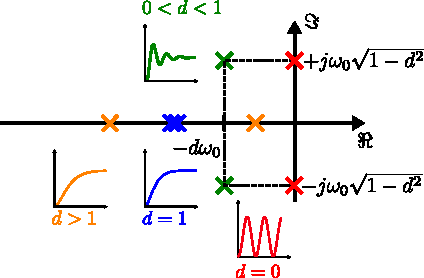
\includegraphics[width=0.6\linewidth]{Abbildungen/Modellbildung/PDF/PT2gliedpn.pdf}
		\caption{Qualitatives Pol- Nullstellen Diagramm des Verzögerungsgliedes 2ter-Ordnung für konjugiert komplexe und reelle Polpaare und deren Sprungantworten}
		\label{fig:pt2gliedpn}
	\end{figure}
	%
	%
	\item Sprungantwort im Zeitbereich: Hierfür muss zunächst eine Fallunterscheidung getroffen werden
	%
	\begin{equation*}
	\begin{aligned}
	%
	0<d<1 \rightarrow H(s)\,\laplace\,h(t)&=\\
	K_{\text{p}}\left[1-\frac{1}{\sqrt{d^{2}-1}}\right.&\left.\cdot e^{-d\omega_{0}t}\cdot\sin\left(\left(\omega_{0}\sqrt{d^{2}-1}\right)t+\text{arccos}(d)\right)\right]\\
	%
	d>1 \rightarrow H(s)\,\laplace\,h(t)&= K_{\text{p}}\left(1-\frac{T_{1}}{T_{1}-T_{2}}e^{-\frac{t}{T_{1}}}+\frac{T_{2}}{T_{1}-T_{2}}e^{-\frac{t}{T_{2}}}\right)\\
	%
	d=1 \rightarrow H(s)\,\laplace\,h(t)&= K_{\text{p}}\left(1-e^{-\frac{t}{T}}\left(1+\frac{t}{T}\right)\right)\\
	%
	d=0 \rightarrow H(s)\,\laplace\,h(t)&= K_{\text{p}}\left(1-\cos\left(\omega_{0}t\right)\right)
	%
	\end{aligned}
	\end{equation*}
	%
	\begin{figure}[h]
		\centering
		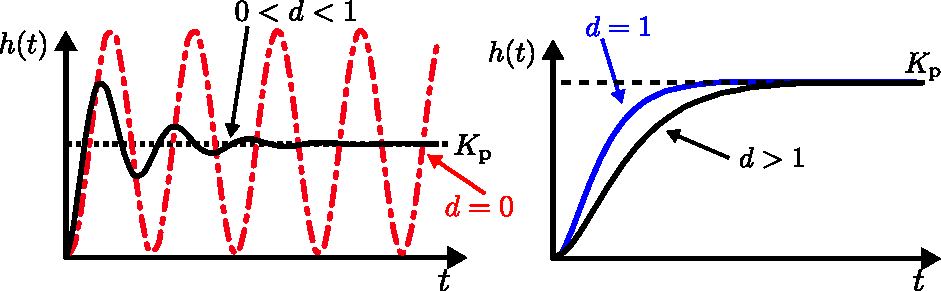
\includegraphics[width=0.9\linewidth]{Abbildungen/Modellbildung/PDF/PT2gliedSprung.pdf}
		\caption{Qualitative Sprungantworten des Verzögerungsglied 2ter-Ordnung}
		\label{fig:pt2gliedsprung}
	\end{figure}
	%
	\item Frequenzgang, Amplitudengang, Phasengang
	%
	\begin{equation*}
	\begin{aligned}
	%
	G(j\omega)&=\frac{K_{\text{p}}}{\frac{(j\omega)^{2}}{\omega_{0}^{2}}+2d\frac{j\omega}{\omega_{0}}+1}\\
	%
	&=\frac{K_{\text{p}}}{1-\frac{\omega^{2}}{\omega_{0}^{2}}+j2d\frac{\omega}{\omega_{0}}}=\frac{K_{\text{p}}\left[1-\frac{\omega^{2}}{\omega_{0}^{2}}\right]-jK_{\text{p}}\left[2d\frac{\omega}{\omega_{0}}\right]}{\left[1-\frac{\omega^{2}}{\omega_{0}^{2}}\right]^{2}+\left[2d\frac{\omega}{\omega_{0}}\right]^{2}}\\
	%
	|G(j\omega)|_{\text{dB}}&=20\lg|G(j\omega)|=20\lg\left(\frac{K_{\text{p}}}{\sqrt{\left[1-\frac{\omega^{2}}{\omega_{0}^{2}}\right]^{2}+\left[2d\frac{\omega}{\omega_{0}}\right]^{2}}}\right)\\
	%
	&=20\lg\left(K_{\text{p}}\right)-20\lg\left(\sqrt{\left[1-\frac{\omega^{2}}{\omega_{0}^{2}}\right]^{2}+\left[2d\frac{\omega}{\omega_{0}}\right]^{2}}\right)\\
	%
	\angle G(j\omega)&=\arctan\left(\frac{-\left[2d\frac{\omega}{\omega_{0}}\right]}{\left[1-\frac{\omega^{2}}{\omega_{0}^{2}}\right]}\right)=-\arctan\left(\frac{\left[2d\frac{\omega}{\omega_{0}}\right]}{\left[1-\frac{\omega^{2}}{\omega_{0}^{2}}\right]}\right)
	%
	\end{aligned}
	\end{equation*}
	%
	\item Bodediagramm
	%
	\begin{figure}[h]
		\centering
		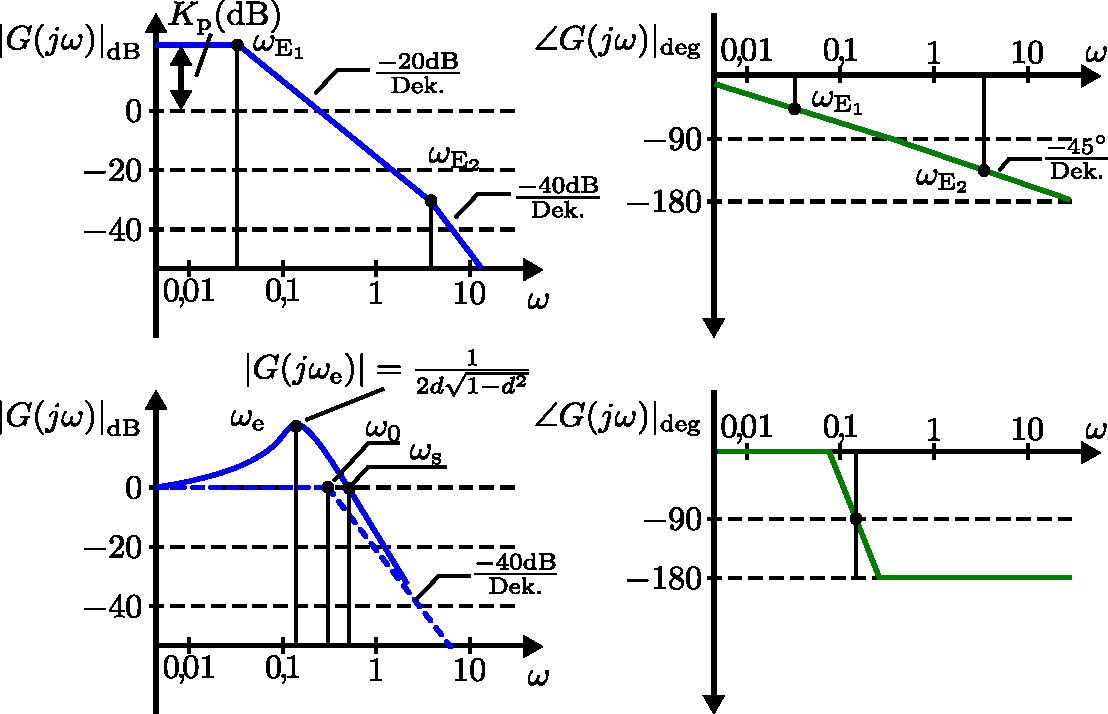
\includegraphics[width=0.9\linewidth]{Abbildungen/Modellbildung/PDF/PT2gliedBode.pdf}
		\caption{Qualitatives Bodediagramm des Verzögerungsglied 2-Ordnung}
		\label{fig:pt2gliedbode}
	\end{figure}
	%
	Anmerkungen zum Bodediagramm: Der Amplituden- und Phasengang ist je nach Dämpfung unterschiedlich:
	\begin{itemize}
		\item $0<d<1$ \textbf{Konjugiert komplexes Polpaar}: Das Verhalten im Bodediagramm ist vergleichbar mit der Resonanz beim Reihenschwingkreis, die Amplitude wird durch den elektrischen Widerstand in der Schaltung begrenzt. Hier ist die Dämpfung $d$ der entscheidende Faktor. Der asymptotische Amplitudengang knickt bei $\omega_{\text{E}}=\omega_{0}$ um $\frac{-40\text{dB}}{Dek.}$ ab. Der tatsächliche Amplitudengang ist in Abbildung~\ref{fig:pt2gliedbode} links unten dargestellt. Die Resonanzüberhöhung entsteht bei $\omega=\omega_{\text{e}}\neq\omega_{0}$. Der Phasengang ist ebenso vom Dämpfungsbeiwert abhängig, je kleiner der Wert, desto steiler verläuft der Phasengang. Der Phasengang startet bei $0^{\circ}$ und verläuft für $\omega\rightarrow \infty$ gegen $-180^{\circ}$
		% 
		\item $d=1$ \textbf{Doppelter reeller Pol}: Aperiodischer Grenzfall, der asymptotische Amplitudengang knickt bei $\omega=\omega_{0}$ um $\frac{-40\text{dB}}{\text{Dek.}}$ ab. Die Durchtrittskreisfrequenz $\omega_{\text{D}}$ wird durch den Verstärkungsbeiwert $K_{\text{p}}$ und durch die Knickfrequenz $\omega_{\text{E}}$ festgelegt. Die Knickfrequenz $\omega_{\text{E}}$ ist bei einer Dämpfung $d=1$ identisch mit $\omega_{0}$. Der Phasengang verläuft wie beim $\text{PT}_{1}-\text{Glied}$ jedoch mit einer Steigung von $\frac{-90^{\circ}}{\text{Dek.}}$. In Höhe der Knickfrequenz ist die Phase $-90^{\circ}$. Der Phasengang startet bei $0^{\circ}$ und verläuft für $\omega\rightarrow \infty$ gegen $-180^{\circ}$
		%
		\item $d>1$ \textbf{Zwei unterschiedliche reelle Pole}: In diesem Fall lässt sich der Amplitudengang wie bei zwei hintereinander geschalteten  $\text{PT}_{1}-\text{Gliedern}$ realisieren. Das Bedeutet das jedes  $\text{PT}_{1}-\text{Glied}$ einen Beitrag zum Amplitudengang ab der jeweiligen Knickfrequenz $\omega_{\text{E},1}$ von $\frac{-20\text{dB}}{\text{Dek.}}$ liefert. Die Steigungen der einzelnen Anteile addieren sich auf, sodass nach der zweiten Knickfrequenz $\omega_{\text{E},2}$ der Amplitudengang eine negative Steigung von $\frac{-40\text{dB}}{\text{Dek.}}$ aufweist. Gleiches gilt für den Phasengang, welcher sich analog zum $\text{PT}_{1}-\text{Glied}$ realisieren lässt. Es muss beachtet werden, dass sich die Wirkung der beiden Pole auf den Phasengang auch überlagern, was bei sehr nahe aneinander liegenden Polen zu einer Steigung der Phasengangs von bis zu $\frac{-90^{\circ}}{\text{Dek.}}$ führt. Der Phasengang startet bei $0^{\circ}$ und verläuft für $\omega\rightarrow \infty$ gegen $-180^{\circ}$
	\end{itemize}
	%
	\item Symbol bzw. Blockschaltbild
	%
	\begin{figure}[h]
		\centering
		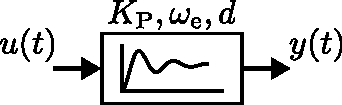
\includegraphics[width=0.3\linewidth]{Abbildungen/Modellbildung/PDF/PT2gliedBlock.pdf}
		\caption{Symbol, Blockschaltbild des Verzögerungsglied 2-Ordnung}
		\label{fig:pt2glied}
	\end{figure}
	%
\end{itemize}
%
\begin{simulation}{}{}
	\begin{itemize}
		\item \textit{Verzögerungsglied 2-Ordnung}
	\end{itemize}
\end{simulation}
%
%%##################################################
%\subsubsection{Verzögerungsglied n-Ordnung (PT$_{\boldsymbol{n}}$-Glied)}
%%##################################################
%%
%Das Verzögerungslied $n$ter-Ordnung, welches eine Verallgemeinerung des PT$_{\boldsymbol{1}}$-Glieds darstellt, lässt sich durch die Aneinanderreihung mehrerer Verzögerungslieder 1ter-Ordnung beschreiben. Mit ihm lassen sich lineare Differentialgleichungen höherer Ordnung abbilden, welche in technischen Prozessen regelmäßig vorkommen.
%%
%\begin{itemize}
%	%
%	\item Funktionalbeziehung im Zeitbereich
%	%
%	\begin{equation*}
%	\begin{aligned}
%	T_{n}\frac{\text{d}^{n}y(t)}{\text{d}t^{n}}+&T_{n-1}\frac{\text{d}^{n-1}y(t)}{\text{d}t^{n-1}}+\cdots+T_{1}\frac{\text{d}y(t)}{\text{d}t}+y(t)=K_{\text{p}}u(t)\\
%	\end{aligned}
%	\end{equation*}
%	%
%	\item Laplacetransformierte und Übergangsfunktion im Bildbereich
%	%
%	\begin{equation*}
%	\begin{aligned}
%	%
%	Y(s)=\frac{K_{\text{p}}}{\left(Ts+1\right)^{n}}U(s),\quad G(s)=\frac{K_{\text{p}}}{\left(Ts+1\right)^{n}},\quad H(s)=\frac{K_{\text{p}}}{s\left(Ts+1\right)^{n}}
%	%
%	\end{aligned}
%	\end{equation*}
%	%
%	\item Sprungantwort im Zeitbereich in Abbildung~\ref{fig:ptngliedsprung}: Für den Spezialfall $n=2$ aus vorheriger Berechnung $d=1$ $H(s)\,\laplace\,h(t)= K_{\text{p}}\left(1-e^{-\frac{t}{T}}\left(1+\frac{t}{T}\right)\right)$
%	%
%	\begin{figure}[h]
%		\centering
%		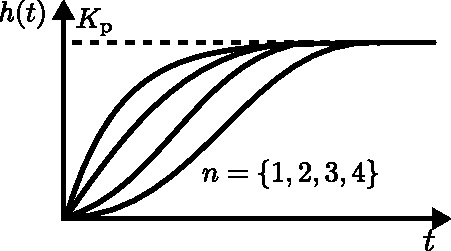
\includegraphics[width=0.4\linewidth]{Abbildungen/Modellbildung/PDF/PTngliedSprung.pdf}
%		\caption{Qualitative Sprungantwort des Verzögerungsglied n-Ordnung}
%		\label{fig:ptngliedsprung}
%	\end{figure}
%	%
%	\item Frequenzgang: Wird hier übersprungen, für den Spezialfall $n=2$ kann er aus dem vorherigen Beispiel des PT$_{\boldsymbol{2}}$-Gliedes berechnet werden. 
%	%
%	\item Bodediagramm: Ergibt sich aus der additiven Überlagerung der einzelnen PT$_{\boldsymbol{1}}$-Gliedern.
%	%
%	\item Symbol bzw. Blockschaltbild
%	%
%	\begin{figure}[h]
%		\centering
%		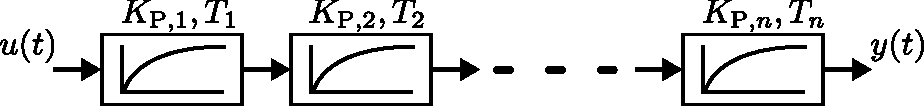
\includegraphics[width=0.7\linewidth]{Abbildungen/Modellbildung/PDF/PTngliedBlock.pdf}
%		\caption{Symbol, Blockschaltbild des Verzögerungsgliedes n-Ordnung}
%		\label{fig:ptnglied}
%	\end{figure}
%	%
%\end{itemize}
%%
%%############################################################################
%\subsubsection{Differenzierglied 1-Ordnung (DT$_{\boldsymbol{1}}$-Glied)}
%%###########################################################################
%%
%Das reale Differenzierglied wird aus der Reihenschaltung eines Differenzierglieds und eines PT$_{\boldsymbol{1}}$-Glieds gebildet.
%%
%\begin{itemize}
%	%
%	\item Funktionalbeziehung im Zeitbereich
%	%
%	\begin{equation*}
%	\begin{aligned}
%	%
%	T_{1}\frac{\text{d}y(t)}{\text{d}t}+y(t)=K_{\text{D}}\frac{\text{d}u(t)}{\text{d}t}
%	%
%	\end{aligned}
%	\end{equation*}
%	%
%	\item Laplacetransformierte und Übergangsfunktion im Bildbereich
%	%
%	\begin{equation*}
%	\begin{aligned}
%	%
%	Y(s)=\frac{K_{\text{D}}s}{\left(T_{1}s+1\right)}U(s),\quad G(s)=\frac{K_{\text{D}}s}{\left(T_{1}s+1\right)},\quad H(s)=\frac{K_{\text{D}}}{\left(T_{1}s+1\right)}
%	%
%	\end{aligned}
%	\end{equation*}
%	%
%	\item Pol- Nullstellen Diagramm im Bildbereich in Abbildung~\ref{fig:dt1gliedpn}: Das $\text{DT}_{1}-\text{Glied}$ besitzt eine Nullstelle im Ursprung $s_{\text{N},1}=0$ und einen Pol bei $s_{\text{P},1}=-\frac{1}{T_{1}}$
%	%
%	\begin{figure}[h]
%		\centering
%		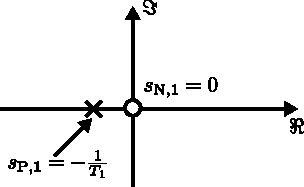
\includegraphics[width=0.4\linewidth]{Abbildungen/Modellbildung/PDF/DT1gliedpn.pdf}
%		\caption{Qualitatives Pol- Nullstellen Diagramm des Differenziergliedes 1ter-Ordnung}
%		\label{fig:dt1gliedpn}
%	\end{figure}
%	%
%	%
%	\item Sprungantwort im Zeitbereich in Abbildung~\ref{fig:dt1gliedsprung}: Laplace Rücktransformation von $H(s)\,\laplace\,h(t)= \frac{K_{\text{p}}}{T_{1}}e^{-\frac{t}{T_{1}}}$
%	%
%	\begin{figure}[h]
%		\centering
%		\includegraphics[width=0.4\linewidth]{Abbildungen/Modellbildung/PDF/DT1gliedSprung.pdf}
%		\caption{Qualitative Sprungantwort des Differenzierglied 1-Ordnung}
%		\label{fig:dt1gliedsprung}
%	\end{figure}
%	%
%	\item Frequenzgang, Amplitudengang, Phasengang
%	%
%	\begin{equation*}
%	\begin{aligned}
%	%
%	G(j\omega)&=\frac{K_{\text{D}}j\omega}{T_{1}j\omega+1}=\frac{K_{\text{D}}j\omega}{T_{1}\omega+1}\cdot\frac{-T_{1}j\omega+1}{-T_{1}j\omega+1}=\frac{K_{\text{D}}\left(j\omega+T_{1}\omega^{2}\right)}{T^{2}_{1}\omega^{2}+1}\\
%	%
%	|G(j\omega)|_{\text{dB}}&=20\lg|G(j\omega)|=20\lg\left(\frac{K_{\text{D}}\omega}{\sqrt{T^{2}_{1}\omega^{2}+1}}\right)\\
%	%
%	&=20\lg\left(K_{\text{D}}\omega\right)-20\lg\left(\sqrt{T_{1}^{2}\omega^{2}+1}\right)\\
%	%
%	\angle G(j\omega)&=\arctan\left(\frac{\frac{K_{\text{D}}\omega}{T^{2}_{1}\omega^{2}+1}}{\frac{K_{\text{D}}T_{1}\omega^{2}}{T^{2}_{1}\omega^{2}+1}}\right)=\arctan\left(\frac{\omega}{T_{1}\omega^{2}}\right)=\arctan\left(\frac{1}{\omega T_{1}}\right)\\
%	\end{aligned}
%	\end{equation*}
%	%
%	\item Bodediagramm in Abbildung~\ref{fig:dt1gliedbode}: Der Amplitudengang startet bei $-\infty$ und besitzt eine positive Steigung von $\frac{+20\text{dB}}{\text{Dek.}}$ identisch zum D-Glied. Die Durchtrittskreisfrequenz $\omega_{\text{D}}$ ergibt sich aus der Verstärkung  $K_{\text{D}}$. Durch den Anteil des $\text{PT}_{1}-\text{Gliedes}$ knickt der Amplitudengang an der Eckfrequenz $\omega_{E}$, da hier ein Beitrag von $\frac{-20\text{dB}}{\text{Dek.}}$ von hinzukommt. In Summe wird der Amplitudengang ab dieser Frequenz invariant gegenüber weiteren Frequenzerhöhungen. Der Phasengang beginnt bei $+90^{\circ}$, identisch wie im Falle des D-Gliedes und fällt durch den Anteil des  $\text{PT}_{1}-\text{Gliedes}$ auf $0^{\circ}$ für $\omega\rightarrow\infty$. An der Eckfrequenz $\omega_{E}$ beträgt die Phase $+45^{\circ}$.
%	%
%	\begin{figure}[ht]
%		\centering
%		\includegraphics[width=0.9\linewidth]{Abbildungen/Modellbildung/PDF/DT1gliedBode.pdf}
%		\caption{Qualitatives Bodediagramm des Differenzierglied 1-Ordnung}
%		\label{fig:dt1gliedbode}
%	\end{figure}
%	%
%	\item Symbol bzw. Blockschaltbild
%	%
%	\begin{figure}[ht]
%		\centering
%		\includegraphics[width=0.45\linewidth]{Abbildungen/Modellbildung/PDF/DT1gliedBlock.pdf}
%		\caption{Symbol, Blockschaltbild des Differenzierglied 1-Ordnung}
%		\label{fig:dt1glied}
%	\end{figure}
%	%
%\end{itemize}
%
%######################################################################
% Erläuzterung zu den Rechenregeln einfügen
%######################################################################
%
\begin{Summary}{}{}
	\begin{itemize}
		\item \textit{Berechnen und zeichnen Sie $\angle G(j\omega)$ und $|G(j\omega)|_{\text{dB}}$ eines IT$_{\boldsymbol{1}}$-Gliedes.}
		\item \textit{Berechnen und zeichnen Sie $\angle G(j\omega)$ und $|G(j\omega)|_{\text{dB}}$ eines PT$_{\boldsymbol{3}}$-Gliedes.}
		\item \textit{Berechnen und zeichnen Sie $\angle G(j\omega)$ und $|G(j\omega)|_{\text{dB}}$ der Reihenschaltung eines PT$_{\boldsymbol{1}}$-Gliedes mit einem Totzeitglied.}
	\end{itemize}
\end{Summary}
%
\newpage
%
%#####################################################
\subsection{Nichtlineare Übertragungsglieder}
%#####################################################
%
Zusätzlich zu den linearen Grundgliedern existieren noch eine Reihe von nichtlineare Gliedern die in vielen Standard-Regelkreisen eingesetzt werden \cite{Foellinger94,Landes00}. Diese sollen im folgenden zusammengefasst werde 
%
\begin{figure}[h]
	%
	\begin{subfigure}[c]{\textwidth}
		\begin{minipage}{0.5\textwidth}
			\begin{itemize}
				\item Kennlinienglied
			\end{itemize}
		\end{minipage}\hfill
		\begin{minipage}{0.5\textwidth}
			\centering
			\includegraphics[width=0.7\textwidth]{Abbildungen/Modellbildung/PDF/Kennlinienglied.pdf}
		\end{minipage}
	\end{subfigure}
	%
	\vspace{1cm}
	%
	\begin{subfigure}[c]{\textwidth}
		\begin{minipage}{0.5\textwidth}
			\begin{itemize}
				\item Magnetisierungskennlinie
			\end{itemize}
		\end{minipage}\hfill
		\begin{minipage}{0.5\textwidth}
			\centering
			\includegraphics[width=0.65\textwidth]{Abbildungen/Modellbildung/PDF/Magnetisierungskurve.pdf}
		\end{minipage}
	\end{subfigure}
	%
	\vspace{1cm}
	%
	\begin{subfigure}[c]{\textwidth}
		\begin{minipage}{0.5\textwidth}
			\begin{itemize}
				\item Zweipunktschalter 
			\end{itemize}
		\end{minipage}
		\begin{minipage}{0.5\textwidth}
			\centering
			\includegraphics[width=0.65\textwidth]{Abbildungen/Modellbildung/PDF/Zweipunktschalter.pdf}
		\end{minipage}
	\end{subfigure} 
	%
	\vspace{1cm}
	%
	\begin{subfigure}[c]{\textwidth}
		\begin{minipage}{0.5\textwidth}
			\begin{itemize}
				\item Zweipunktschalter mit Hysterese
			\end{itemize}
		\end{minipage}\hfill
		\begin{minipage}{0.5\textwidth}
			\centering
			\includegraphics[width=0.65\textwidth]{Abbildungen/Modellbildung/PDF/ZweipunktschalterHyst.pdf}
		\end{minipage}
	\end{subfigure} 
	%
	\vspace{1cm}
	%
	\begin{subfigure}[c]{\textwidth}
		\begin{minipage}{0.5\textwidth}
			\begin{itemize}
				\item Betragsbildner
			\end{itemize}
		\end{minipage}\hfill
		\begin{minipage}{0.5\textwidth}
			\centering
			\includegraphics[width=0.7\textwidth]{Abbildungen/Modellbildung/PDF/Betragsglied.pdf}
		\end{minipage}
	\end{subfigure}
	%
	\vspace{1cm}
	%
	\begin{subfigure}[c]{\textwidth}
		\begin{minipage}{0.5\textwidth}
			\begin{itemize}
				\item Multiplizier Glied
			\end{itemize}
		\end{minipage}\hfill
		\begin{minipage}{0.5\textwidth}
			\centering
			\includegraphics[width=0.5\textwidth]{Abbildungen/Modellbildung/PDF/Multiplizierer.pdf}
		\end{minipage}
	\end{subfigure}
	% 
\end{figure}
%
\newpage
%
\begin{figure}[h]
	%
	\begin{subfigure}[c]{\textwidth}
		\begin{minipage}{0.5\textwidth}
			\begin{itemize}
				\item Dividier Glied
			\end{itemize}
		\end{minipage}
		\begin{minipage}{0.5\textwidth}
			\centering
			\includegraphics[width=0.5\textwidth]{Abbildungen/Modellbildung/PDF/Dividierer.pdf}
		\end{minipage}
	\end{subfigure} 
	%
	\vspace{1cm}
	%
	\begin{subfigure}[c]{\textwidth}
		\begin{minipage}{0.5\textwidth}
			\begin{itemize}
				\item Quadrier Glied
			\end{itemize}
		\end{minipage}\hfill
		\begin{minipage}{0.5\textwidth}
			\centering
			\includegraphics[width=0.5\textwidth]{Abbildungen/Modellbildung/PDF/Quadrierer.pdf}
		\end{minipage}
	\end{subfigure} 
	%
	\vspace{1cm}
	%
	\begin{subfigure}[c]{\textwidth}
		\begin{minipage}{0.5\textwidth}
			\begin{itemize}
				\item Wurzel Glied
			\end{itemize}
		\end{minipage}\hfill
		\begin{minipage}{0.5\textwidth}
			\centering
			\includegraphics[width=0.5\textwidth]{Abbildungen/Modellbildung/PDF/Ratifizierer.pdf}
		\end{minipage}
	\end{subfigure} 
	%
	\vspace{1cm}
	%
	\begin{subfigure}[c]{\textwidth}
		\begin{minipage}{0.5\textwidth}
			\begin{itemize}
				\item Invertierer
			\end{itemize}
		\end{minipage}\hfill
		\begin{minipage}{0.5\textwidth}
			\centering
			\includegraphics[width=0.5\textwidth]{Abbildungen/Modellbildung/PDF/Invertierer.pdf}
		\end{minipage}
	\end{subfigure}
\end{figure}
%
\vspace{-20pt}
%
%##############################################################
\section{Experimentelle Bestimmung der Systemparameter}
\label{sec:experimental}
%##############################################################
%
Bis wurde untersucht, wie durch mathematische Modelle, Systeme beschrieben werden können. Diese wurden anhand von Differenzialgleichungen formuliert und danach analysiert. Eine weitere Möglichkeit ist es, die Systemparameter und somit das Modell des Systems aus einer Reihe von Messwerten der Systemantwort auf geschickt gewählte Eingangssignale zu schätzen \cite{Foellinger94}. Hierzu sollen nur dynamische Systeme betrachtet werden, die auch durch die vorher erläuterten Grundglieder dargestellt werden können.
%
%##########################################
\subsubsection{Allgemeine Vorgehensweise:}
%##########################################
%
Um das Systemverhalten zu ermitteln, wird die Reaktion des Systems auf eine Änderung des Eingang ausgewertet. Zunächst muss hierfür einige wesentliche Schritte durchlaufen werden, die im Folgenden beschrieben werden:
%
\begin{itemize}
%
\item Festlegung eines geeigneten Testsignals
%
	\begin{itemize}
	\item Systemidentifikation im Zeitbereich.
		%
		\begin{itemize}
		\item Wird in der Regel mittels Sprungfunktion vorgenommen. Die Sprungfunktion bietet eine starke Anregung, lässt sich einfach realisieren und ermöglicht es die Übergangsfunktion des Systems zu berechnen.
		\item Für rotierende Systeme (elektrische Maschinen) ist der Sprung nicht geeignet, da die Drehzahl nicht zu hoch werden darf. Hier können auch Rechteck Impulse genutzt werden.
		\item Falls das untersuchte System Beschränkungen in der Verstellgeschwindigkeit besitzt (Ventile) ist eine weitere Möglichkeit die Nutzung einer Rampenfunktion. 
		\end{itemize}
		%
	\item Systemidentifikation im Frequenzbereich.
		%
		\begin{itemize}
		\item Nutzung einer Sinusschwingung und somit Auswertung des Frequenzgangs des Systems. 
		\end{itemize}
	\end{itemize}
%
\item Festlegung des Modellansatzes.
%
	\begin{itemize}
		\item Berücksichtigung von Vorkenntnissen über das System.
		%
		\begin{itemize}
			\item Idealerweise sind die physikalischen Gleichungen bekannt und lediglich die Parameter müssen geschätzt werden.
			\item Ein Modell annehmen ($\text{PT}_{1}$, $\text{PT}_{2}$ mit/ohne Totzeit) und die Reaktion des Systems mit diesem vergleichen.
			\item Angleichen des Modells an die Ergebnisse im fortlaufenden Prozess.
		\end{itemize}
		%
	\end{itemize}
%
\item Wahl des Gütekriteriums.
%
	\begin{itemize}
	%
	\item Minimierung von Modellfehlern mittels Gütefunktion z.B durch die Lösung eine Optimierungsproblems (Leased Squares)
	%	
	\end{itemize}
%
\item Berechnung der Parameter
%
\end{itemize}
%
Es handelt sich hierbei um eine iterative Vorgehensweise, welche sich Schrittweise an die tatsächlichen Parameter des Systems annähert. Die Parameterschätzung ist somit ein Art Regelkreis, bei dem der reale Systemausgang mit dem des Modells verglichen und über einen Schätzalgorithmus, die Parameteränderungen zurückgeführt werden (siehe Abbildung\ref{fig:parameterschaetzen}).
%
\begin{figure}[h]
	\centering
	\includegraphics[width=0.7\linewidth]{Abbildungen/Modellbildung/PDF/ParameterSchaetzung.pdf}
	\caption{Wirkungsplan zur Schätzung von Systemparametern \cite{Foellinger94}}
	\label{fig:parameterschaetzen}
\end{figure}
%
\begin{simulation}{}{}
	\begin{itemize}
		\item \textit{Parameterschätzung mit \textbf{fminsearch()}} \copyright MATLAB
	\end{itemize}
\end{simulation}
%
%###################################################################
\subsection{Bestimmung des Übertragungsverhaltens von Grundgliedern}
%##################################################################
%
Nach dieser allgemeinen Übersicht sollen nun im Anschluss einige konkrete Beispiele folgen. Es werden allerdings nur einfache Fälle betrachtet; Bestimmung der Parameter von $\text{PT}_{1}$,$\text{PT}_{2}$ Gliedern über graphische Auswertung der Sprungantwort.
%
%#################################################################
\subsubsection{Anfangs- und Endwerte der Sprungantwort}
%#################################################################
%
Aus dem Endwert- bzw. Anfangswertsatz kann anhand der Sprungantwort ein spezifisches Verhalten ermittelt werden. Ausgehend von der Übertragungsfunktion
%
\begin{equation*}
\begin{aligned}
G(s)=\frac{b_{q}s^{q}+b_{q-1}s^{q-1}+\cdots+b_{1}s+b_{0}}{a_{n}s^{n}+a_{n-1}s^{n-1}+\cdots+a_{1}s+a_{0}}\\
\end{aligned}
\end{equation*}
%
ergibt sich der Endwertsatz zu:
%
\begin{equation*}
\begin{aligned}
\lim\limits_{t\rightarrow\infty}h(t)=\lim\limits_{s\rightarrow 0}sH(s)=\lim\limits_{s\rightarrow 0}G(s)=\frac{b_{0}}{a_{0}}.\\
\end{aligned}
\end{equation*}
%
Der Anfangswertsatz zu:
%
\begin{equation*}
\begin{aligned}
\lim\limits_{t\rightarrow 0}h(t)=\lim\limits_{s\rightarrow \infty}sH(s)=\lim\limits_{s\rightarrow \infty}G(s).\\
\end{aligned}
\end{equation*}
%
Um den Anfangswertsatz zu bestimmen, kann es notwendig sein die Regeln von l'Hospital anzuwenden und Zähler so wie Nenner getrennt voneinander abzuleiten. Grundsätzlich können unterschiedliche Verhalten der Sprungantwort so Klassifiziert werden.
%
\begin{itemize}
	\item Integrales Verhalten $\lim\limits_{t\rightarrow\infty}h(t)=\infty$
	\item Proportionales Verhalten $\lim\limits_{t\rightarrow\infty}h(t)=K_{\text{P}}$
	\item Differenzierendes Verhalten $\lim\limits_{t\rightarrow\infty}h(t)=0$
\end{itemize}
%
%#################################################################
\subsubsection{Strecken mit PT$_{\boldsymbol{1}}$ Verhalten}
%#################################################################
%
Strecken die ein PT$_{\boldsymbol{1}}$ Verhalten aufweisen, können mittels der Übertragungsfunktion
%
\begin{equation*}
\begin{aligned}
%
G(s)&=\frac{\hat{K}_{\text{P}}}{\hat{T}_{1}s+1}%
%
\end{aligned}
\end{equation*}
%
dargestellt werden. Hierbei signalisiert der $\{\,\hat{}\,\}$ Operator, dass es sich nur um einen geschätzten und nicht um den Wahren Wert handelt. Beide Werte lassen sich aus der Sprungantwort des Systems rekonstruieren, wie in Abbildung~\ref{fig:experimpt1} dargestellt.
%
\begin{figure}[h]
	\centering
	\includegraphics[width=0.45\linewidth]{Abbildungen/Modellbildung/PDF/ExperimentelPT1.pdf}
	\caption{Schätzung der Systemparameter eine PT$_{\boldsymbol{1}}$-Glieds \cite{Foellinger94}}
	\label{fig:experimpt1}
\end{figure}
%
$\hat{K}_{\text{P}}$ ergibt sich aus der stationären Verstärkung bzw. dem Endwert. $\hat{T}_{\text{1}}$ wiederum, ergibt sich aus dem Schnittpunkt der Tangente an den linearen Teil die Anstiegskurve und dem stationären Endwert. Je nachdem wie hoch der Rauschanteil des Signals ist ergeben sich bessere oder schlechtere Werte bei der graphischen Bestimmung.
%
%#################################################################
\subsubsection{Allgemeine Verzögerungsglieder}
%#################################################################
%https://www.eit.hs-karlsruhe.de/mesysto/teil-a-zeitkontinuierliche-signale-und-systeme/uebertragungsglieder-der-regelungstechnik/minimalphasige-systeme-und-allpaesse/allpaesse.html
%
Verallgemeinert man nun die Betrachtung auf Übertragungsglieder erster Ordnung, so ergeben sich auch sprungfähige Systeme der Form
%
\begin{equation*}
\begin{aligned}
%
G(s)&=\hat{K}_{\text{P}}\frac{\hat{T}_{\text{V}}s+1}{\hat{T}_{1}s+1}%
%
\end{aligned}
\end{equation*}
%
Mit der Vorhaltezeitkonstante $\hat{T}_{\text{V}}$ und der bereits bekannten Verzögerungszeitkonstante $\hat{T}_{\text{1}}$. Im Zeitbereich lässt sich dieses Übertragungsglied folgendermaßen darstellen
%
\begin{equation*}
\begin{aligned}
%
h(t)&=\hat{K}_{\text{P}}\left[1-\left(1-\frac{\hat{T}_{\text{V}}}{\hat{T}_{\text{1}}}\right)e^{-\frac{t}{\hat{T}_{1}}}\right].
%
\end{aligned}
\end{equation*}
%
Aus dieser Gleichung lässt sich zudem der Anfangs- und Endwert der Sprungantwort direkt ermitteln.
%
\begin{equation*}
\begin{aligned}
%
\lim\limits_{t\rightarrow 0}h(t)&=\hat{K}_{\text{P}}\left[1-\left(1-\frac{\hat{T}_{\text{V}}}{\hat{T}_{\text{1}}}\right)\underbrace{e^{-\frac{0}{\hat{T}_{1}}}}_{=1}\right] = \frac{\hat{K}_{\text{P}}\hat{T}_{\text{V}}}{\hat{T}_{1}}\\	
%
\lim\limits_{t\rightarrow \infty}h(t)&=\hat{K}_{\text{P}}\left[1-\left(1-\frac{\hat{T}_{\text{V}}}{\hat{T}_{\text{1}}}\right)\underbrace{e^{-\frac{\infty}{\hat{T}_{1}}}}_{=0}\right] = \hat{K}_{\text{P}}
%
\end{aligned}
\end{equation*}
%
In Abbildung~\ref{fig:experimallpass} lässt sich sehr gut die Wirkung der Nullstelle im Zeitverhalten. So kompensiert die Nullstelle das Verhalten der Polstelle für $\hat{T}_{\text{V}}>\hat{T}_{1}$ und lässt das Glied differenzierend wirken.
%
\begin{figure}[h]
	\centering
	\includegraphics[width=0.5\linewidth]{Abbildungen/Modellbildung/PDF/ExperimentelAllpass.pdf}
	\caption{Schätzung von Systemparametern beliebiger Systeme 1 Ordnung \cite{Foellinger94}}
	\label{fig:experimallpass}
\end{figure}
%
Besonders diese Eigenschaften macht man sich in Regelkreisen als sogenanntes Kompensationsglied zu nutze. Doch sollte erwähnt werden, das die Nullstelle ein Überschwingen im Regelkreis erzeugen kann. Auch wenn nur reelle Polstellen vorzufinden sind.
%
%%#################################################################
%\subsubsection{Übertragungsglieder mit Überschwingen ohne periodisches Schwingen}
%%#################################################################
%%
%Untersucht man Übertragungsglieder die nur reele Pole und eine Nullstelle besitzen, so kann des Überschwingens auch auf Übertragungsglieder höherer Nennerordnung übertragen werden.
%%
%\begin{equation}
%\begin{aligned}
%%
%G(s)&=\hat{K}_{\text{P}}\frac{\hat{T}_{\text{V}}s+1}{\left(\hat{T}_{1}s+1\right)\left(\hat{T}_{2}s+1\right)}\label{eq:nullstelle}%
%%
%\end{aligned}
%\end{equation}
%%
%\begin{figure}[h]
%	\centering
%	\includegraphics[width=0.4\linewidth]{Abbildungen/Modellbildung/PDF/ExperimentelNullstelle.pdf}
%	\caption{Überschwingen bei reellwertigen Polen}
%	\label{fig:experimnull}
%\end{figure}
%%
%Wie aus Abbildung~\ref{fig:experimnull} ersichtlich existieren drei unterschiedliche Verhalten
%%
%\begin{itemize}
%	\item $\hat{T}_{\text{V}}>\max\{\hat{T}_{1},\hat{T}_{2}\}$, System schwingt über und konvergiert von oben gegen den Endwert.
%	\item $\hat{T}_{\text{V}}<\max\{\hat{T}_{1},\hat{T}_{2}\}$, Wirkung der Nullstelle führt zum verlangsamen des Systems
%	\item $\hat{T}_{\text{V}}=0$, PT$_{\boldsymbol{2}}$-Verhalten mit reellen Polen.
%\end{itemize}
%%
%Auch die Anfangssteigung der Systemantwort wird durch die Nullstelle beeinflusst. So reduziert sich die Anfangssteigung mit der Reduktion von $\hat{T}_{\text{V}}$ und erreicht den Wert 0 für $\hat{T}_{\text{V}}=0$.
%%
%\begin{Aufgaben}{}{}
%	\begin{itemize}
%		\item \textit{Berechnung der Anfangssteigung $\frac{\text{d}h(t)}{\text{d}t}$ mittels Gleichung~\ref{eq:nullstelle}}
%	\end{itemize}
%\end{Aufgaben}
%
%#################################################################
\subsubsection{Strecken mit PT$_{\text{N}}$ Verhalten}
%#################################################################
%
In der Praxis existieren oft Strecken, welche als Summe von mehreren Verzögerungsgliedern 1-Ordnung dargestellt werden können. Nun sind die Zeitkonstanten in der Regel unterschiedlich, was aber nicht differenziert analysiert werden kann. Stattdessen wird eine sogenannte Summenzeitkonstante gebildet und die unterschiedlichen Zeitkonstante in einer abgebildet.
%
\begin{equation*}
\begin{aligned}
%
G(s)&=\frac{\hat{K}_{\text{P}}}{\left(\hat{T}_{1}s+1\right)\left(\hat{T}_{2}s+1\right)\cdots\left(\hat{T}_{\text{N}}s+1\right)}\approx\frac{\hat{K}_{\text{P}}}{\left(\hat{T}s+1\right)^{\text{N}}}e^{-T_{t}s}%
%
\end{aligned}
\end{equation*}
%
Bei der experimentellen Bestimmung geht es hauptsächlich darum eine möglichst gute Summenzeitkonstante und Systemtotzeit zu ermitteln. Die Verfahren zur Bestimmung der Systemparameter von PT$_{\text{N}}$ Verhalten sind zum Teil sehr Aufwendig und sollen hier nur kurz skizziert werden.
%
\begin{itemize}
%
\item Wendetangentenverfahren: Bestimmung einer Tangente im linearen Teil der Sprungantwort. Ermittlung von Anstiegszeit $\hat{t}_{\text{g}}$ und Verzugszeit $\hat{t}_{\text{u}}$. Approximation mittels PT$_{\text{1}}$T$_{\text{t}}$-Glied.
%
\item Strejc Verfahren: Bestimmung zweier Punkte $(\hat{t}_{1},\hat{h}_{1}),(\hat{t}_{2},\hat{h}_{2})$ im linearen Bereich der Sprungantwort. Ermittlung der Systemparameter anhand einer Entwurfsformel. 
%
\begin{equation*}
\begin{aligned}
%
\hat{T} &= \frac{\hat{t}_{2}-\hat{t}_{1}}{\ln\left(\frac{\hat{K}_{\text{P}}-\hat{h}_{1}}{\hat{K}_{\text{P}}-\hat{h}_{2}}\right)}\\
%
\hat{T}_{t}&= \hat{T}\ln\left(1-\frac{\hat{h}_{2}}{\hat{K}_{\text{P}}}\right)+\hat{t}_{2}
%
\end{aligned}
\end{equation*}
%
Bestimmung der stationären Verstärkung aus dem Endwert und Approximation mittels PT$_{\text{1}}$T$_{\text{t}}$-Glied.
%
\item Zeitprozentwertverfahren nach Schwarz \cite{Zacher17}: Es werden drei Prozentwerte der Sprungantwort bei $10\%$, $50\%$ und $90\%$ des Endwertes gebildet.
%
\end{itemize}
%
%\begin{Aufgaben}{}{}
%	\begin{itemize}
%		\item \textit{Rechenbeispiel Strejc-Verfahren}
%	\end{itemize}
%\end{Aufgaben}
%
\begin{figure}[h]
	\centering
	\includegraphics[width=0.45\linewidth]{Abbildungen/Modellbildung/PDF/ExperimentelPTn.pdf}
	\caption{Sprungantwort eines PT$_{N}$-Glieds und die zu schätzenden Parameter \cite{Foellinger94}}
	\label{fig:experimptn}
\end{figure}
%
%#################################################################
\subsubsection{Strecken mit schwingungsfähigem PT$_{2}$ Verhalten}
%#################################################################
%
Handelt es sich bei der Sprungantwort eines Systems um eine abklingende Schwingung, so existieren auch hierfür Verfahren, um die Parameter der Kurve zu ermitteln. Hierbei werden sowohl die Frequenz der Schwingung als auch die Reduktion der Amplitude der Schwingung zu Bestimmung herangezogen, wie in Abbildung~\ref{fig:experimpt2} dargestellt.
%
\begin{figure}[ht!]
	\centering
	\includegraphics[width=0.55\linewidth]{Abbildungen/Modellbildung/PDF/ExperimentelPT2.pdf}
	\caption{Sprungantwort eines PT2-Glieds und die zu schätzenden Parameter \cite{Foellinger94}}
	\label{fig:experimpt2}
\end{figure}
%
Bei schwingungsfähigen Systemen muss zudem ein Toleranzband für die Erreichung des stationären Endwerts festgelegt werden. Dieses liegt in der Regel bei $3\%$ oder $5\%$ bezogen auf den Endwert. Die Strecke wird durch folgende angenäherte Übertragungsfunktion dargestellt.
%
\begin{equation*}
\begin{aligned}
%
G(s)&=\frac{\hat{K}_{\text{P}}}{\frac{s^{2}}{\hat{\omega_{0}}^{2}}+2\hat{d}\frac{s}{\hat{\omega_{0}}}+1}%
%
\end{aligned}
\end{equation*}
%
Folgende Parameter werden benötigt
%
\begin{itemize}
	\item Anregelzeit $\hat{t}_{\text{An}}$ ist erreicht, wenn die Sprungantwort das erste Mal den Endwert schneidet. 
	\item Ausregelzeit $\hat{t}_{\text{Aus}}$ ist erreicht, wenn die Sprungantwort in den $3\%$ oder $5\%$ Schlauch um den Endwert eintritt.
	\item Periodendauer $\hat{T}_{\text{P}}$, ermittelt sich aus der Eigenschwingung der Systemantwort.
	\item Amplituden $\hat{A}_{0},\hat{A}_{1},\hat{A}_{2},\hat{A}_{3},\hat{A}_{4},\cdots,\hat{A}_{\text{N}}$
	\item Prozentuale Überschwingweite $\hat{u}$
\end{itemize}
%
Nach Auswertung der Sprungantwort sind die Dämpfung $\hat{d}$ und die Kreisfrequenz $\hat{\omega}_{0}$ gesucht. Mittels folgender Formeln lassen sich nun die Parameter bestimmen \cite{Foellinger94}.
%
\begin{equation*}
\begin{aligned}
%
\hat{K}_{\text{P}}&=h_{\infty}, \quad &&j\hat{\omega}_{e}=j\hat{\omega}_{0}\sqrt{1-\hat{d}^{2}},\,\,\forall \hat{d} \in \{0<\hat{d}<1\}\\
%%
\hat{u}&=\frac{\hat{A}_{k+1}}{\hat{A}_{k}}, &&\hat{d}=\frac{1}{\sqrt{1 + \left[\frac{\pi}{\ln(\hat{u})}\right]^{2}}}\\
%%
\hat{\omega}_{0}&=\frac{2\pi}{\hat{T}_{\text{P}}\sqrt{1 - \hat{d}^{2}}}, &&\hat{T}_{\text{P}}=\frac{2\pi}{\hat{\omega}_{0}}\sqrt{1 - \hat{d}^{2}}
%
\end{aligned}
\end{equation*}
%
%#######################################################################################
\section{Modellvereinfachung}
%#######################################################################################
%
Bis zum jetzigen Zeitpunkt wurde die Regelstrecke durch ein mathematisches Modell dargestellt oder durch Messung der Systemantwort bestimmt. Dies kann jedoch unter Umständen zu sehr komplexen, oder auch nichtlinearen Blöcken führen. Im folgenden soll gezeigt werden, wie diese Modelle vereinfacht werden können, um sie leichter in der Regelung einzusetzen.
%
%#######################################################################################
\subsection{Normierung}
%#######################################################################################
%
Ziel der Normierung ist es die Einheiten aus den Systemgleichungen zu eliminieren und einen einheitlichen Zahlenraum für physikalische Größen zu erhalten. Besonders beim Einsatz in Rechnergestützten Programmen oder einer Regelung per Microcomputer, verhilft die Normierung den Wertebereich der Regel- und Stellgrößen bestmöglich zu nutzen. Denn je nach Variablen Typ (z.B. 8 Bit Integer) kann es leicht zu einem Überlauf kommen. Nutzen wir wieder das Beispiel der Gleichstrommaschine, so würden die Normierten Größen sich bezogen auf ihren Maximalwert oder Nennwert ergeben \cite{SML14}
%
\begin{equation*}
\begin{aligned}
%
\frac{i_\text{A}}{I_{\text{A,Nenn}}}=\tilde{i_\text{A}} \quad \text{entspricht} \quad \frac{u_\text{A}}{U_{\text{A,Nenn}}}=\tilde{u_\text{A}} \quad \text{mit} \quad -1\leq \{i_\text{A},u_\text{A}\} \leq +1
%
\end{aligned}
\end{equation*}
%
Alle Größen sind ab diesem Zeitpunkt auf die Basis SI-Einheiten normiert und somit dimensionslos. Hierdurch wird jedoch auch eine bessere Vergleichbarkeit zwischen unterschiedlichen Maschinensätzen unterschiedlicher Größe gegeben, da ja die Struktur der Maschine gleich bleibt.
%
\begin{Aufgaben}{}{}
	\begin{itemize}
		\item \textit{Normierung der Gleichstrommaschine}
		\item \textit{Normierung einer Wechselstromimpedanz}
	\end{itemize}
\end{Aufgaben}
%
%#######################################################################################
\subsection{Linearisierung}
%#######################################################################################
%
Viele in der Praxis vorkommende Systeme haben nichtlineares Verhalten. Jedoch bietet die Regelungstechnik für LZI-Glieder ein wesentliches breiteres Spektrum an Methoden an. Des Weiteren zeigt sich in vielen Fällen, dass es ausreicht ein System in der Nähe eines Arbeitspunktes zu betrachten und es um diesen Arbeitspunkt zu linearisieren \cite{Lunze10,MSF05}. Dabei ist der Arbeitspunkt als ein beliebiger stationärer Zustand des Systems zu verstehen. Dies kann zum Beispiel der stationäre Endwert der Sprungantwort eines Systems sein, welcher sich aus der Übertragungsfunktion
%
\begin{equation*}
\begin{aligned}
%
G(s)=\frac{b_{q}s^{q}+b_{q-1}s^{q-1}+\cdots+b_{1}s+b_{0}}{a_{n}s^{n}+a_{n-1}s^{n-1}+\cdots+a_{1}s+a_{0}}\\%\bigg\rvert_{G(s\rightarrow 0)}\\
%
\end{aligned}
\end{equation*}
%
und der Anwendung des Endwertsatzes ergibt
%
\begin{equation*}
\begin{aligned}
%
\lim\limits_{t\rightarrow\infty }h(t)=h_{\infty}=\frac{a_{0}}{b_{0}}.
%
\end{aligned}
\end{equation*}
%
Im Weiteren gehen wir davon aus, dass wir einen beliebigen stationären Zustand eines Systems, definiert durch $y_{0},u_{0}$ haben.  
%
\subsubsection{Bestimmung von stationären Zuständen aus dem Wirkungsplan}
%
Per Definition sind alle zeitveränderlichen Größen im stationären Zustand konstant. Ein Sonderfall wäre der Integrator, welcher gesondert betrachtet werden muss, da sich für einen konstanten Eingang $u_{0}$ kein konstanter Ausgang $y_{0}$ einstellt. Die Vorgehensweise zur Bestimmung der stationären Werte erfolgt nach folgendem Muster:
%
\begin{itemize}
	\item Eingänge aller Integrator Glieder zu 0 setzen.
	\item In anderen Blöcken $s=0$ setzen.
	\item Stationäre Gleichungen aus dem Wirkungsplan ablesen.
	\item Sollwerte der Ausgangsgröße einsetzen.
	\item Berechnung der übrigen Größen.
\end{itemize}
%
Exemplarisch soll dies Anhand des RL-Glieds und dessen Wirkschaltplan dargestellt werden (siehe Abbildung~\ref{fig:stationaer})
%
\begin{figure}[h]
	\centering
	\includegraphics[width=1\linewidth]{Abbildungen/Modellbildung/PDF/WirkschaltplanStationaer.pdf}
	\caption{Berechnung des stationären Wertepaares anhand des Wirkschaltplans}
	\label{fig:stationaer}
\end{figure}
%
\begin{Aufgaben}{}{}
	\begin{itemize}
		\item \textit{Berechnung des stationären Zustandes aus dem Wirkschaltplan}
	\end{itemize}
\end{Aufgaben}
%
\subsubsection{Berechnung des linearisierten Systems}
%
Durch den stationären Punkt wird eine Tangente gelegt welcher einer Näherung des nichtlinearen Verhaltens durch eine lineare Funktion entspricht (vlg. Abbildung~\ref{fig:Linearisierung}).
%
\begin{figure}[h]
	\centering
	\includegraphics[width=0.45\linewidth]{Abbildungen/Modellbildung/PDF/Linearisierung.pdf}
	\caption{Linearisierung einer nichtlinearen Funktion durch eine Geradenapproximation}
	\label{fig:Linearisierung}
\end{figure}\\
%
Formal wird die Linearisierung durch eine Approximation mittels Taylorreihe beschrieben 
%
\begin{equation*}
\begin{aligned}
%
f(u)\approx \sum_{n=0}^{\infty}\frac{1}{n!} \frac{\text{d}f^{n}(u)}{\text{d}u^{n}}\bigg\rvert_{u=u_{0}}\left(u-u_{0}\right)^{n},
%
\end{aligned}
\end{equation*}
%
welches jedoch nach dem linearen Glied abgebrochen wird und sich somit auf folgende Gleichung reduziert
%
\begin{equation*}
\begin{aligned}
%
f(u)\approx f(u_{0})+\underbrace{\frac{\text{d}f(u)}{\text{d}u}\bigg\rvert_{u=u_{0}}}_{m}\underbrace{\left(u-u_{0}\right)}_{\Delta u},
%
\end{aligned}
\end{equation*}
%
Dies ist jedoch nur möglich wenn die Funktion im Arbeitspunkt stetig differenzierbar ist. D.h. Knickstellen oder Sprünge können nicht als Arbeitspunkt genutzt werden.
%
Durch die Verschiebung in ein neues Koordinatensystem ist das linearisierte Modell nur relativ zum Arbeitspunkt aussagekräftig. Um diese Eigenschaft im Blockschaltbild zu berücksichtigen müssen die Arbeitspunkte mit in das Modell einfließen, um nach außen hin vergleichbare Werte zum nichtlinearen Verhalten zu erhalten (vgl. Abbildung~\ref{fig:LinBlock}).
%
\begin{figure}[h!]
	\centering
	\includegraphics[width=0.5\linewidth]{Abbildungen/Modellbildung/PDF/LinearisierungBlock.pdf}
	\caption{Darstellung der Linearisierung im Blockschaltbild}
	\label{fig:LinBlock}
\end{figure}
%
Dieser Ansatz lässt sich auch für Funktionen mehrerer Veränderlicher realisieren. Als Beispiel soll ein System mit mehreren Eingängen und einem Ausgang dienen. Die Taylor Reihe wird nun partiell für sämtliche Variablen entwickelt und nach dem ersten Glied abgebrochen. 
%
\begin{equation*}
\begin{aligned}
%
f(u_{1},..., u_{\text{N}})\approx f(u_{10},..., u_{N0})+\sum_{\nu=1}^{\text{N}}\frac{\partial f(\cdot)}{\partial u_{\nu}}\bigg\rvert_{u_{\nu}=u_{\nu 0}}\left(u_{\nu}-u_{\nu0}\right)\label{eq:MultiTaylor}
%
\end{aligned}
\end{equation*} 
%
Wie aus vorherigen Kapiteln bekannt ist die Summenbildung in Gleichung~\ref{eq:MultiTaylor} linear. Für das linearisierte System gilt somit das Überlagerungsprinzip.  
%
\begin{simulation}{}{}
	\begin{itemize}
		\item \textit{Linearisierung am Beispiel des Fliehkraftpendel nach \cite{MSF05}, Seite 54}
	\end{itemize}
\end{simulation}
%
Zusammenfassend ergeben sich folgende Besonderheiten:
%
\begin{itemize}
	\item Das Koordinatensystem des linearisierten Modells hat seinen Ursprung im Arbeitspunkt $(y_{0},u_{0})$ und seine Variablen sind nun relative Größen $(\Delta y,\Delta u)$.
	%
	\item Je weiter wir uns vom Arbeitspunkt entfernen, um so schlechter approximiert das lineare, das ursprüngliche Modell.
	%
	\item Der Wirkschaltplan muss die Koordinatenverschiebung berücksichtigen.
	%
	\item Bei Linearisierung von Funktion mehrerer Veränderlicher gilt für die einzelnen Approximationen das Linearistätsprinzip.
	%
	\item Lineare Übertragungsglieder bleiben erhalten, da sie durch die Taylor Reihe exakt beschrieben werden.
\end{itemize}
%
%#######################################################################################
\subsection{Wirkungsplanvereinfachung}
%#######################################################################################
%
Übertragungsfunktionen ermöglichen ein einfaches Rechnen mit dynamischen Systemen, welche aus mehreren Teilsystemen bestehen. Ziel ist es die Gesamtübertragungsfunktion bspw. der Regelstrecke zu finden, um den Regler hierfür auslegen zu können. Die Drei am häufigsten vorkommenden Verschaltungen von Übertragungsfunktionen werden im folgenden vorgestellt (nach \cite{Lunze10}).
%
\subsubsection{Reihenschaltung von Übertragungsfunktionen}
%
Bei der Reihenschaltung von Übertragungsfunktionen wirkt der jeweilige Ausgang des vorherigen Blockes auf den Eingang des nachgeschalteten, wie in Abbildung~\ref{fig:Reiheschaltung} dargestellt. D.h. es gilt zunächst für die Teilübertragungsfunktionen
%
\begin{equation}
\begin{aligned}
%
Y_{1}(s)&=G_{1}(s)U_{1}(s)\\
Y_{2}(s)&=G_{2}(s)U_{2}(s)\label{eq:Reihenschaltung}
%
\end{aligned}
\end{equation} 
%
\begin{figure}
	\centering
	\includegraphics[width=0.85\linewidth]{Abbildungen/Modellbildung/PDF/RechenregelnMult.pdf}
	\caption{Regeln für die Reihenschaltung von Übertragungsfunktionen nach \cite{Lunze10}}
	\label{fig:Reiheschaltung}
\end{figure}
%
Aus der Verschaltung in Abbildung~\ref{fig:Reiheschaltung}, wird ersichtlich das
%
\begin{equation*}
\begin{aligned}
%
Y(s)&=Y_{2}(s)\\
U_{2}(s)&=Y_{1}(s)\\
U_{1}(s)&=U(s)
%
\end{aligned}
\end{equation*} 
%
Setzt man diesen Zusammenhang in Gleichung~\ref{eq:Reihenschaltung} ein, erhält man das Ergebnis der Reihenschaltung.
%
\begin{equation*}
\begin{aligned}
%
Y(s)&=G_{1}(s)G_{2}(s)U(s)
%
\end{aligned}
\end{equation*} 
%
Diese besagt, dass eine Reihenschaltung von zwei Übertragungsfunktionen einer Multiplikation gleicht. Würde man dies mit Zeitfunktionen realisieren, so müssten die beiden Gewichtsfunktionen mit dem Faltungsintegral verrechnet werden.
%
\subsubsection{Parallelschaltung von Übertragungsfunktionen}
%
Bei der Parallelschaltung von Übertragungsfunktionen wirken die jeweiligen Ausgänge der einzelnen Blöcke in Summe auf den Gesamtausgang, wie in Abbildung~\ref{fig:Parallelschaltung} dargestellt. 
%
\begin{figure}[ht!]
	\centering
	\includegraphics[width=0.85\linewidth]{Abbildungen/Modellbildung/PDF/RechenregelnAddittion.pdf}
	\caption{Regeln für die Parallelschaltung von Übertragungsfunktionen nach \cite{Lunze10}}
	\label{fig:Parallelschaltung}
\end{figure}
%
D.h. es gilt zunächst für die Teilübertragungsfunktionen
%
\begin{equation}
\begin{aligned}
%
Y(s)&=Y_{1}(s)+Y_{2}(s)\\
U(s)&=U_{1}(s)=U_{2}(s)\\
Y_{1}(s)&=G_{1}(s)U_{1}(s)\\
Y_{2}(s)&=G_{2}(s)U_{2}(s)\label{eq:Parallelschaltung}
%
\end{aligned}
\end{equation} 
%
Aus der Verschaltung in Abbildung~\ref{fig:Parallelschaltung} und Gleichung~\ref{eq:Parallelschaltung}, wird ersichtlich das
%
\begin{equation*}
\begin{aligned}
%
Y(s)=\left(G_{1}(s)+G_{2}(s)\right)U(s)
%
\end{aligned}
\end{equation*} 
%
Das Ergebnis besagt, dass eine Parallelschaltung von zwei Übertragungsfunktionen einer Addition gleicht. Im Zeitbereich würden die gleichen Regeln für die Gewichtsfunktionen gelten.
%
\subsubsection{Schaltung von Übertragungsfunktionen mit Rückführung}
%
Werden verschiedene Übertragungsfunktionen in einem geschlossenen Regelkreis zusammengeführt, so entstehen oft Rückführungen. Da die Regelgröße zudem gemessen werden muss, kann es vorkommen das, dass Messglied in der Rückführung auftaucht, wie in Abbildung~\ref{fig:Rückführung} dargestellt.
%
\begin{figure}[ht!]
	\centering
	\includegraphics[width=0.85\linewidth]{Abbildungen/Modellbildung/PDF/RechenregelnRueckkopplung.pdf}
	\caption{Regeln für die Rückführung von Übertragungsfunktionen nach \cite{Lunze10}}
	\label{fig:Rückführung}
\end{figure}
%
Für die Signale lässt sich folgende Beziehung aufstellen
%
\begin{equation*}
\begin{aligned}
%
Y(s)&=Y_{1}(s)\\
U_{1}(s)&=U(s)-Y_{2}(s)
%
\end{aligned}
\end{equation*} 
%
Woraus sich ergibt das
%
\begin{equation*}
\begin{aligned}
%
Y(s)&=\left(U(s)-Y_{2}(s)\right)G_{1}(s)\\
Y(s)&=\left(U(s)-Y(s)G_{2}(s)\right)G_{1}(s)\\
Y(s)&=G_{1}(s)U(s)-G_{2}(s)G_{1}(s)Y(s)\\
Y(s)&=\frac{G_{1}(s)}{1+G_{2}(s)G_{1}(s)}U(s)
%
\end{aligned}
\end{equation*}
%
Im Zeitbereich würde man hingegen nur eine nicht sehr anschauliche implizite Gleichung bekommen. Es existieren noch weitere Umformungsregeln welche genutzt werden können, um Blöcke zusammenzufassen Verknüpfungspunkte zu verschieben, oder Additionen zu vertauschen. In Abbildung~\ref{fig:WirkVerinfachung} sind einige wichtige Rechenregeln zusammengefasst.
%
\begin{figure}
	\centering
	\includegraphics[width=1\linewidth]{Abbildungen/Modellbildung/PDF/Blockschaltbildvereinfachung.pdf}
	\caption{Regeln für das Umformen von Blockschaltbildern nach \cite{Foellinger94,Lunze10}}
	\label{fig:WirkVerinfachung}
\end{figure}
%
\begin{Summary}{}{}
	\begin{itemize}
		\item Nutzen Sie Abbildung~\ref{fig:vorsteuerung} und überlegen Sie, welche Veränderung das Signal $u_{\text{v}}(t)$ erfährt, wenn es am Ausgang wirken soll.
		\item Überprüfen Sie die Linearitätsbedingung für die Parallelschaltung in Abbildung~\ref{fig:Parallelschaltung}.
	\end{itemize}
\end{Summary}